%\pdfoutput=1
\documentclass[12pt,a4paper,reqno]{amsart}
\newcommand\hmmax{0}
\newcommand\bmmax{0}
\usepackage{amssymb}
\usepackage{amscd}
\usepackage[pdftex,pdfpagelabels]{hyperref}
\usepackage{enumerate}
\usepackage{comment}
%\usepackage{psfig}
\usepackage{graphicx}
\usepackage{cleveref}
\usepackage{siunitx}
\usepackage{tikz-cd}
\usepackage{stix}
\usepackage{bm}
\DeclareMathAlphabet\mathbfcal{LS2}{stixcal}{b}{n}
\numberwithin{equation}{section}

%\usepackage{mathabx}


\usepackage{mathtools}%                  http://www.ctan.org/pkg/mathtools
\usepackage[tableposition=top]{caption}% http://www.ctan.org/pkg/caption
\usepackage{booktabs,dcolumn}%           http://www.ctan.org/pkg/dcolumn + http://www.ctan.org/pkg/booktabs

% Lighter notation.
%\newcommand*\mc[1]{\multicolumn{1}{c}{#1}}
%\newcommand*\tupref[2]{\href{http://math.mit.edu/~primegaps/tuples/admissible_#1_#2.txt}{\num{#2}}}



%\DeclareMathOperator*\Kl{Kl} (commented because yield bad display for  \Kl_q %replaced with \newcommand... )
%\DeclareMathOperator*\FT{FT} (commented because yield bad display for \FT_q
%replaced with \newcommand...)

\DeclareMathOperator*\swan{swan}
\DeclareMathOperator*\cond{cond}
\DeclareMathOperator*\Gal{Gal}

\newcommand{\FT}{\mathrm{FT}}
\newcommand{\Kl}{\mathcal{K}\ell}
% Setup for ``caption''.
%\DeclareCaptionLabelSeparator{separation}{:\quad}
%\captionsetup{
  %font=small,
  %labelfont=sc,
  %labelsep=separation,
  %width=0.8\textwidth
%}

\DeclareFontFamily{OT1}{rsfs}{}
\DeclareFontShape{OT1}{rsfs}{n}{it}{<-> rsfs10}{}
\DeclareMathAlphabet{\mathscr}{OT1}{rsfs}{n}{it}

\addtolength{\textwidth}{3 truecm}
\addtolength{\textheight}{1 truecm}
\setlength{\voffset}{-.6 truecm}
\setlength{\hoffset}{-1.3 truecm}

\theoremstyle{plain}

\newtheorem{theorem}{Theorem}[section]
%\newtheorem{theorem}[theorem]{Theorem}
\newtheorem{proposition}[theorem]{Proposition}
\newtheorem{lemma}[theorem]{Lemma}
\newtheorem{corollary}[theorem]{Corollary}
\newtheorem{conjecture}[theorem]{Conjecture}
\newtheorem{heuristic}[theorem]{Heuristic}
\newtheorem{principle}[theorem]{Principle}
\newtheorem{question}[theorem]{Question}
\newtheorem{problem}[theorem]{Problem}
\newtheorem{claim}[theorem]{Claim}

\theoremstyle{definition}

%\newtheorem{roughdef}[subsection]{Rough Definition}
\newtheorem{definition}[theorem]{Definition}
\newtheorem{remark}[theorem]{Remark}
\newtheorem{remarks}[theorem]{Remarks}
\newtheorem{example}[theorem]{Example}
\newtheorem{examples}[theorem]{Examples}
%\newtheorem{problem}[subsection]{Problem}
%\newtheorem{question}[subsection]{Question}

\renewcommand\P{\mathbb{P}}
\newcommand\E{\mathbb{E}}
\newcommand\Var{\mathrm{Var}}
\newcommand\R{\mathbb{R}}
\newcommand\Z{\mathbb{Z}}
\newcommand\F{\mathbf{F}}
\newcommand\N{\mathbb{N}}
\newcommand\n{\mathbf{n}}
\renewcommand\a{\mathbf{a}}
\renewcommand\b{\mathbf{b}}
\renewcommand\j{\mathbf{j}}
\renewcommand\k{\mathbf{k}}
\renewcommand\v{\mathbf{v}}
\renewcommand\t{\mathbf{t}}
\renewcommand\r{\mathbf{r}}
\renewcommand\l{\mathbf{l}}
\newcommand\X{\mathbf{X}}
\newcommand\T{\mathbf{T}}
\newcommand\Y{\mathbf{Y}}
\newcommand\A{\mathbf{A}}
\newcommand\W{\mathbf{W}}
\newcommand\C{\mathbb{C}}
\newcommand\Q{\mathbb{Q}}
\renewcommand\Re{{\operatorname{Re}}}
\renewcommand\Im{{\operatorname{Im}}}
\newcommand\Log{{\operatorname{Log}}}
\newcommand\lcm{{\operatorname{lcm}}}
\renewcommand\gcd{{\operatorname{gcd}}}
\newcommand\eps{\varepsilon}
\newcommand\tuple{{\mathcal B}}
\newcommand\excess{{\mathcal{E}}}

\renewcommand{\mod}{\bmod}

\parindent 0mm
\parskip   5mm


\begin{document}

\title{Decomposing a factorial into large factors}


\author{...}
\address{???}
\email{???}

\author{Terence Tao}
\address{UCLA Department of Mathematics, Los Angeles, CA 90095-1555.}
\email{tao@math.ucla.edu}
\subjclass[2020]{11A51}

\begin{abstract}  Let $t(N)$ denote the largest number such that $N!$ can be expressed as the product of $N$ numbers greater than or equal to $t(N)$.
The bound $t(N)/N = 1/e-o(1)$ was apparently established in unpublished work of Erd\H{o}s, Selfridge, and Straus; but the proof is lost.  Here we obtain the more precise asymptotic 
$$ \frac{t(N)}{N} = \frac{1}{e} - \frac{c_0}{\log N} + O\left( \frac{1}{\log^{1+c} N} \right)$$
for an explicit constant $c_0 = 0.3044190\dots$ and some absolute constant $c>0$, answering a question of Erd\H{o}s and Graham.  With numerical assistance, we also establish several conjectures of Guy and Selfridge concerning effective estimates of this quantity, for instance establishing $t(N) \geq N/3$ for $N \geq 43632$, with the threshold shown to be best possible.\end{abstract}


\maketitle

%%%%%%%%%%%%%%%%%%%%%%%%%%%%%%%%%%%%%%%%%%%%%%%%%

\section{Introduction}

Given a natural number $M$, define a \emph{factorization} of $M$ to be a finite multiset $\tuple$ such that the product
$$ \prod \tuple \coloneqq \prod_{a \in \tuple} a$$
(where the product is counted with multiplicity) is equal to $M$; more generally, define a \emph{subfactorization} of $M$ to be a finite multiset $\tuple$ such that $\prod \tuple$ divides $M$.  Given a threshold $t$, we say that a multiset $\tuple$ is \emph{$t$-admissible} if $a \geq t$ for all $a \in \tuple$.  For a given natural number $N$, we then define $t(N)$ to be the largest $t$ for which there exists a $t$-admissible factorization $\tuple$ of $N!$ of cardinality $|\tuple|=N$.  

\begin{example}\label{nine}  The multiset
  $$ \{ 3,3,3,3,4,4,5,7,8\}$$
  is a $3$-admissible factorization of 
$$ \prod \{ 3,3,3,3,4,4,5,7,8\} = 3^4 \times 4^2 \times 5 \times 7 \times 8 = 9!$$
of cardinality 
$$|\{ 3,3,3,3,4,4,5,7,8\}| = 9,$$
 hence $t(9) \geq 3$.  One can check that no $4$-admissible factorization of $9!$ of this cardinality exists, hence $t(9) = 3$.
\end{example}

It is easy to see that $t(N)$ is non-decreasing in $N$, (any cardinality $N$ factorization of $N!$ can be extended to a cardinality $N+1$ factorization of $(N+1)!$ by adding $N+1$ to the multiset).  The first few elements of the sequence $t(N)$ are
$$ 1,1,1,2,2,2,2,2,3,3,3,3,3,4, \dots$$
(\href{https://oeis.org/A034258}{OEIS A034258}). The values of $t(N)$ for $N \leq 79$ were computed in \cite{guy}, and the values for $N \leq 200$ can be extracted from \href{https://oeis.org/A034259}{OEIS A034259}, which describes the inverse sequence to $t$.

When the factorial $N!$ is replaced with an arbitrary number, this problem is essentially the bin covering problem, which is known to be NP-hard; see e.g., \cite{bincover}.  However, as we shall see in this paper, the special structure of the factorial (and in particular, the profusion of factors at the ``tiny primes'' $2,3$) make it more tractable than the general case.

\begin{remark}\label{subfac}  One can equivalently define $t(N)$ as the greatest $t$ for which there exists a $t$-admissible \emph{subfactorization} of $N!$ of cardinality \emph{at least} $N$.  This is because every such subfactorization can be converted into a $t$-admissible factorization of cardinality exactly $N$ by first deleting elements from the subfactorization to make the cardinality $N$, and then multiplying one of the elements of the subfactorization by a natural number to upgrade the subfactorization to a factorization.  This ``relaxed'' formulation of the problem turns out to be more convenient for both theoretical analysis of $t(N)$ and numerical computations.
\end{remark}

By combining the obvious lower bound
\begin{equation}\label{obvious}
 \prod \tuple \geq t^{|\tuple|}
\end{equation}
for any $t$-admissible multiset $\tuple$ with Stirling's formula \eqref{stirling}, we obtain the trivial upper bound
\begin{equation}\label{trivial} \frac{t(N)}{N} \leq \frac{(N!)^{1/N}}{N} = \frac{1}{e} + O\left( \frac{\log N}{N}\right)
\end{equation}
for $N \geq 2$; see \Cref{fig1}.  In \cite[p.75]{erdos-graham} it was reported that an unpublished work of Erd\H{o}s, Selfridge, and Straus established the asymptotic
\begin{equation}\label{t1}
  \frac{t(N)}{N} = \frac{1}{e} + o(1)
\end{equation}
(first conjectured in \cite{erdos-71}) and asked if one could show the bound
\begin{equation}\label{Tbound}
   \frac{t(N)}{N} \leq \frac{1}{e} - \frac{c}{\log N}
\end{equation}
for some constant $c>0$ (problem {\#}391 in \url{https://www.erdosproblems.com}; see also \cite[Section B22, p. 122--123]{guy}); it was also noted that similar results were obtained in \cite{algr77} if one restricted the $a_i$ to be prime powers.  However, as later reported in \cite{erdos-96}, Erd\H{o}s ``believed that Straus had written up our proof [of \eqref{t1}]. Unfortunately Straus suddenly died and no trace was ever found of his notes. Furthermore, we never could reconstruct our proof, so our assertion now can be called only a conjecture''.   In \cite{guy} the lower bound $\frac{t(N)}{N} \geq \frac{1}{4}$ was established for sufficiently large $N$, by rearranging powers of $2$ and $3$ in the obvious factorization $1 \times 2 \times \dots \times N$ of $N!$.  A variant lower bound of the asymptotic shape $\frac{t(N)}{N} \geq \frac{3}{16}-o(1)$ obtained by rearranging only powers of $2$, and which is superior for medium values of $N$, can also be found in \cite{guy}.  The following conjectures in \cite{guy} were also made:
\begin{enumerate}
\item One has $t(N) \leq N/e$ for $N \neq 1,2,4$.
\item One has $t(N) \geq \lfloor 2N/7 \rfloor$ for $N \neq 56$.
\item One has $t(N) \geq N/3$ for $N \geq 3 \times 10^5$.  (It was also asked if the threshold $3 \times 10^5$ could be lowered.) 
\end{enumerate}

\begin{figure}
  \centering
  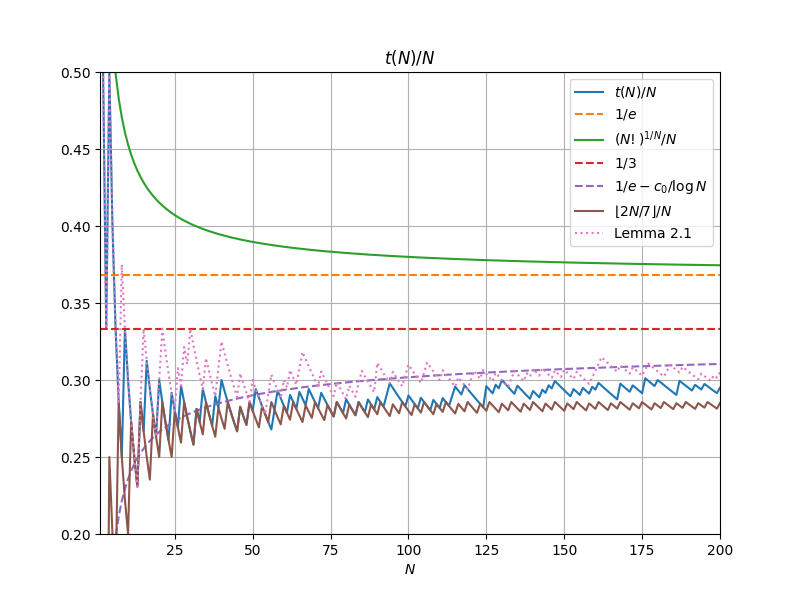
\includegraphics[width=0.8\textwidth]{newplot_200.png}
  \caption{The function $t(N)/N$ (blue) for $N \leq 200$, using the data from \href{https://oeis.org/A034258}{OEIS A034258}, as well as the trivial upper bound $(N!)^{1/N}/N$ (green), the improved upper bound from \Cref{upper-crit} (pink), which is asymptotic to \eqref{asym} (purple), and the function $\lfloor 2N/7 \rfloor/N$ (brown), which is a lower bound for $N \neq 56$ \cite{guy}.  \Cref{main} implies that $t(N)/N$ is asymptotic to \eqref{asym} (purple), which in turn converges to $1/e$ (orange).  The threshold $1/3$ (red) is permanently crossed at $N=43632$. {\bf TODO: relabel image to reflect new lemma numbering}}\label{fig1}
  \end{figure}
  
  \begin{figure}
    \centering
    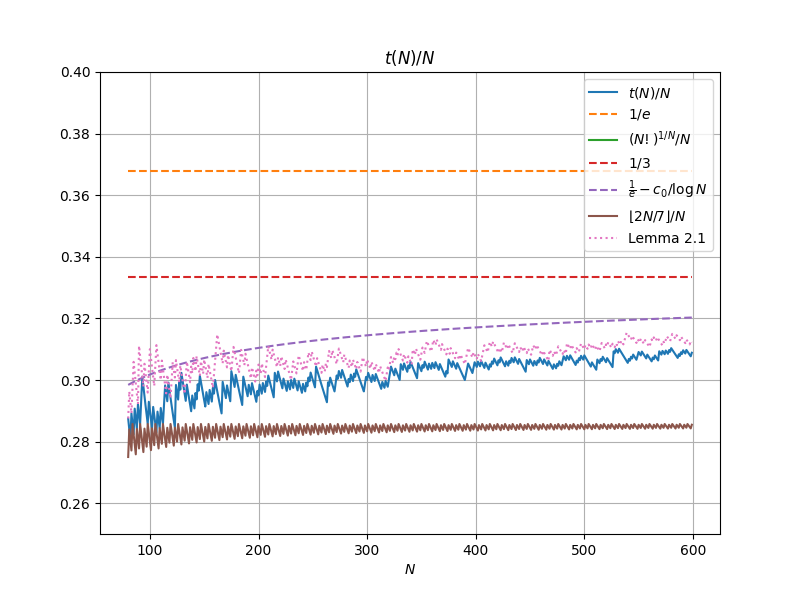
\includegraphics[width=0.8\textwidth]{newplot_600_all.png}
    \caption{A continuation of \Cref{fig1} to the region $80 \leq N \leq 599$. }\label{fig1-alt}
  \end{figure}
  
In this paper we answer all of these questions.

\begin{theorem}[Main theorem]\label{main} Let $N$ be a natural number.
\begin{itemize}
\item[(i)] If $N \neq 1,2,4$, then $t(N) \leq N/e$.
\item[(ii)]  If $N \neq 56$, then $t(N) \geq \lfloor 2N/7 \rfloor$.
\item[(iii)]  If $N \geq 43632$, then $t(N) \geq N/3$.  The threshold $43632$ is best possible.
\item[(iv)]  For large $N$, one has
  \begin{equation}\label{asym}
    \frac{t(N)}{N} = \frac{1}{e} - \frac{c_0}{\log N} + O\left( \frac{1}{\log^{1+c} N} \right)
  \end{equation}
for some constant $c>0$, where $c_0$ is the explicit quantity
\begin{equation}\label{c0-def}
  \begin{split}
  c_0 &\coloneqq \frac{1}{e} \int_0^1 f_e(x)\ dx \\
  &= 0.3044190\dots
\end{split}
\end{equation}
and for any $\alpha>0$, $f_\alpha \colon (0,\infty) \to \R$ denotes the piecewise smooth function
\begin{equation}\label{falpha-def} 
  f_\alpha(x) \coloneqq \left\lfloor \frac{1}{x} \right\rfloor \log \frac{\lceil 1/\alpha x \rceil}{1/\alpha x}.
\end{equation}
In particular, \eqref{t1} and \eqref{Tbound} hold.
\end{itemize}
\end{theorem}

For future reference, we observe the simple bounds
\begin{equation}\label{falpha-bound}
 \begin{split}
   0 \leq f_\alpha(x) &\leq \frac{1}{x} \log \frac{1/\alpha x+1}{1/\alpha x}\\
&= \frac{1}{x} \log\left( 1 + \alpha x \right) \\
&\leq \alpha
\end{split}
\end{equation}
for all $x>0$; in particular, $f_\alpha$ is a bounded function.  It however has an oscillating singularity at $x=0$; see \Cref{fig:mean}.

In \Cref{c0-app} we give some details on the numerical computation of the constant $c_0$.

\begin{remark}\label{old} In a previous version \cite{tao} of this manuscript, the weaker bounds
  $$ \frac{1}{e} - \frac{O(1)}{\log N} \leq \frac{t(N)}{N} \leq \frac{1}{e} - \frac{c_0+o(1)}{\log N}$$
were established, which were enough to recover \eqref{t1}, \eqref{Tbound}, and \Cref{main}(i). 
\end{remark}  

\begin{figure}
  \centering
  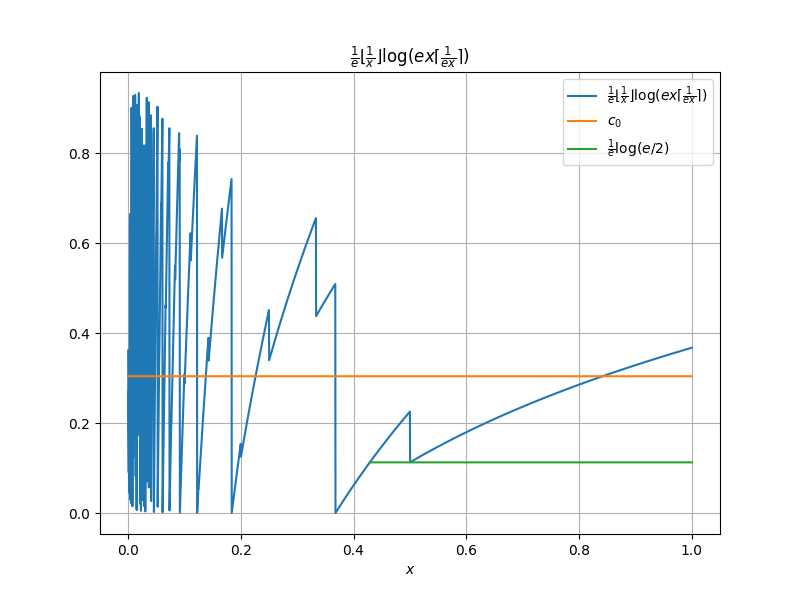
\includegraphics[width=0.8\textwidth]{integ.png}
  \caption{The piecewise continuous function $x\mapsto \frac{1}{e} f_e(x)$, together with its mean value $c_0 = 0.3044190\dots$ and the upper bound $\frac{\log(1+ex)}{ex}$.  The function exhibits an oscillatory singularity at $x=0$ similar to $\sin \frac{1}{x}$ (but it is always nonnegative and bounded). Informally, the function $f_e$ quantifies the difficulty that large primes in the factorization of $N!$ have in becoming slightly larger than $N/e$ after multiplying by a natural number.}\label{fig-mean}
\end{figure}

As one might expect, the proof of \Cref{main} proceeds by a combination of both theoretical analysis and numerical calculations.  Our main tools to obtain upper and lower bounds on $t(N)$ can be summarized as follows:

\begin{itemize}
  \item In \Cref{greedy-sec}, we discuss \emph{greedy algorithms} to construct subfactorizations, that provide quickly computable, though suboptimal, lower bounds on $t(N)$ for small and medium values;
  \item In \Cref{linprog-sec}, we present a \emph{linear programming} (or \emph{integer programming}) method that provides quite accurate upper and lower bounds on $t(N)$ for small and medium values of $N$;
  \item In \Cref{accounting-sec}, we introduce an \emph{accounting identity} linking the ``$t$-excess'' of a subfactorization with its ``$p$-surpluses'' at various primes, which provides an reasonable upper bound on $t(N)$ for all $N$, and is discussed in more detail in \Cref{accounting-sec};
  \item In \Cref{approx-sec}, we give \emph{modified approximate factorization} strategy, which provides lower bounds on $t(N)$, that become asymptotically quite efficient.
\end{itemize}

The final approach is significantly more complicated than the other three, but is the only one which gives efficient lower bounds in the asymptotic limit $N \to \infty$.  The key idea is to start with an approximate factorization
$$ N! \approx \left(\prod_{j \in I} j\right)^A$$
for some small natural number $A$ (e.g., $A = \lfloor \log^2 N \rfloor$) and a suitable set $I$ of natural numbers greater than or equal to $t$; there is some freedom to select parameters here, and we will take $I$ to be the natural numbers in $(t, t(1+\sigma)]$ that are coprime to $6$, where $t$ is the target lower bound for $t(N)$ we wish to establish, and $\sigma \coloneqq \frac{3N}{tA}$.  With a suitable choice of $I$, this product contains approximately the right number of copies of $p$ for medium-sized primes $p$; but it has the ``wrong'' number of copies of large primes, and is also constructed to avoid the ``tiny'' primes $p=2,3$.  One then performs a number of alterations to this approximate factorization to correct for the ``surpluses'' or ``deficits'' at various primes $p>3$, using the supply of available tiny primes $p=2,3$ as a sort of ``liquidity pool'' to efficiently reallocate primes in the factorization.  A key point will be that the incommensurability of $\log 2$ and $\log 3$ (i.e., the irrationality of $\log 3/\log 2$) means that the $3$-smooth numbers (numbers of the form $2^n 3^m$) are asymptotically dense (in logarithmic scale), allowing for other factors to be exchanged for $3$-smooth factors with little loss\footnote{The weaker results alluded to in \Cref{old} only used the prime $2$ as a supply of ``liquidity'', and thus encountered inefficiencies due to the inability to ``make change'' when approximating another factor by a power of two.}.

\subsection{Author contributions and data}

This project was initially concieved as a single-author manuscript by Terence Tao, but since the release of the initial preprint \cite{tao}, grew to become a collaborative project organized via the Github repository \cite{github}, which also contains the supporting code and data for the project.  The contributions of the individual authors, according to the CRediT categories at \url{https://credit.niso.org/}, are as follows:

{\bf authors should be arranged in alphabetical order of surname.  }

\begin{itemize}
\item ...
\item Terence Tao: Conceptualization, Formal Analysis, Methodology, Project Administration, Visualization, Writing -- original draft, Writing -- review \& editing.
\end{itemize}

\subsection{Acknowledgments}

TT is supported by NSF grant DMS-2347850.  We thank Thomas Bloom for the web site \url{https://www.erdosproblems.com}, where the author learned of this problem, as well as Bryna Kra and Ivan Pan for  corrections.

{\bf list here all contributors to the project who did not wish to be listed as co-authors.}


\section{Notation and basic estimates}

If $S$ is a statement, we use $1_S$ to denote its indicator, thus $1_S=1$ when $S$ is true and $1_S=0$ when $S$ is false.  If $x$ is a real number, we use $\lfloor x \rfloor$ to denote the greatest integer less than or equal to $x$, and $\lceil x \rceil$ to be the least integer greater than or equal to $x$.

Throughout this paper, the symbol $p$ (or $p'$, $p_1$, $p_2$, etc.) is always understood to be restricted to be prime.  The primes $2,3$ will play a special role in this paper and will be referred to as \emph{tiny primes}. 
Call a natural number \emph{$3$-smooth} if it is the product of tiny primes, i.e., it is of the form $2^n 3^m$ for some natural numbers $n,m$.  Given a positive real number $x$, we use $\lceil x \rceil^{\langle 2,3 \rangle}$ to denote the smallest $3$-smooth number greater than or equal to $x$.  For instance, $\lceil 5 \rceil^{\langle 2,3 \rangle} = 6$ and $\lceil 10 \rceil^{\langle 2,3 \rangle} = 12$. 
For any $L \geq 1$, let $\kappa_L$ be the least quantity such that
\begin{equation}\label{kappa-def}  
  x \leq \lceil x \rceil^{\langle 2,3\rangle} \leq \exp(\kappa_L) x 
\end{equation}
holds for all $x \geq L$. Just from considering the powers of two, we have the trivial upper bound
\begin{equation}\label{kl-triv}
  \kappa_L \leq \log 2.
\end{equation}
In fact $\kappa_L$ decays to zero as $L$ goes to infinity, due to the incommensurability of $\log 2$ and $\log 3$; we quantify this decay in \Cref{power-sec}. 

In practice, $\lceil x \rceil^{\langle 2,3 \rangle}$ will only be slightly larger than $x$; we quantify this in \Cref{power-sec}.

We use $(a,b)$ to denote the greatest common divisor of $a$ and $b$, $a|b$ to denote the assertion that $a$ divides $b$, and $\pi(x) = \sum_{p \leq x} 1$ to denote the usual prime counting function. The effective and asymptotic estimates over primes that we will use are summarized in \Cref{primes-sec}.

We use $\nu_p(a/b) = \nu_p(a)-\nu_p(b)$ to denote the $p$-adic valuation of a positive natural number $a/b$, that is to say the number of times $p$ divides the numerator $a$, minus the number of times $p$ divides the denominator $b$.  For instance, $\nu_2(32/27)=5$ and $\nu_3(32/27)=-3$. 
If one applies a logarithm to the fundamental theorem of arithmetic, one obtains the identity
\begin{equation}\label{ftoa}
  \sum_p \nu_p(r) \log p = \log r
\end{equation}
for any positive rational $r$.  

For a natural number $n$, we can write
\begin{equation}\label{nup-form} 
  \nu_p(n) = \sum_{j=1}^\infty 1_{p^j|n}.
\end{equation}
Upon taking partial sums, we recover Legendre's formula
\begin{equation}\label{legendre}
  \nu_p(N!) = \sum_{j=1}^\infty \left\lfloor \frac{N}{p^j} \right\rfloor = \frac{N - s_p(N)}{p-1}
\end{equation}
where $s_p(N)$ is the sum of the digits of $N$ in the base $p$ expansion.

Given a putative factorization $\tuple$ of $N!$,  
we refer to the quantity $\nu_p\left( \frac{N!}{\prod \tuple} \right)$ as the \emph{$p$-surplus} of $\tuple$ with respect to the target $N!$; if it is negative, we refer to $-\nu_p\left( \frac{N!}{\prod \tuple} \right)$ as the \emph{$p$-deficit}, with the multiset being \emph{$p$-balanced} if the $p$-surplus (or $p$-deficit) is zero.  Thus, a factorization of $N!$ is achieved if and only if one is balanced at every prime $p$, whereas a subfactorization is achieved if one is either in balance or surplus at every prime $p$.

We use the usual asymptotic notation $X = O(Y)$, $X \ll Y$, or $Y \gg X$ to denote an inequality of the form $|X| \leq CY$ for some absolute constant $C$.  We also write $X \asymp Y$ for $X \ll Y \ll X$. For effective estimates, we will use the more precise notation $O_{\leq}(Y)$ to denote any quantity whose magnitude is bounded by exactly at most $Y$. We also use $O_{\leq}(Y)^+$ to denote a quantity of size $O_{\leq}(Y)$ that is in addition non-negative, that is to say it lies in the interval $[0,Y]$.

To bound the factorial, we have the explicit Stirling approximation \cite{robbins}
\begin{equation}\label{stirling}
  N \log N - N + \log \sqrt{2\pi N} + \frac{1}{12N+1} \leq \log N! \leq N \log N - N + \log \sqrt{2\pi N} + \frac{1}{12N},
\end{equation}
valid for all natural numbers $N$. 


\section{Linear programming}\label{linprog-sec}

A surprisingly sharp upper bound on $t(N)$ comes from linear programming.

\begin{lemma}[Linear programming bound]\label{lp-upper}  Let $N$ be an natural number and $1 \leq t \leq N/2$.  Suppose for each prime $p \leq N$, one has a non-negative real number $w_p$ which is weakly non-decreasing in $p$ (thus $w_p \leq w_{p'}$ when $p \leq p'$), and such that
  \begin{equation}\label{pj}
   \sum_p w_p \nu_p(j) \geq 1
  \end{equation}
  for all $t \leq j \leq N$, and such that
  \begin{equation}\label{hyp}
  \sum_p w_p \nu_p(N!) < N.
  \end{equation}
  Then $t(N) < t$.
  \end{lemma}
  
  \begin{proof}
  We first observe that the bound \eqref{pj} in fact holds for all $j \geq t$, not just for $t \leq j \leq N$.  Indeed, if this were not the case, consider the first $j \geq t$ where \eqref{pj} fails.  Take a prime $p$ dividing $j$ and replace it by a prime in the interval $[p/2,p)$ which exists by Bertrand's postulate (or remove $p$ entirely, if $p=2$); this creates a new $j'$ in $[j/2,j)$ which is still at least $t$.  By the weakly decerasing hypothesis on $w_p$, we have
  $$ \sum_p w_p \nu_p(j) \geq \sum_p w_p \nu_p(j')$$
  and hence by the minimality of $j$ we have
  $$ \sum_p w_p \nu_p(j) > 1, $$
  a contradiction.
  
  Now suppose for contradiction that $t(N) \geq t$, thus we have a factorization $N! = \prod_{j \geq t} j^{m_j}$ for some natural numbers $m_j$ summing to $N$.  Taking $p$-valuations, we conclude that
  $$ \sum_{j \geq t} m_j \nu_p(j) \leq \nu_p(N!)$$
  for all $p \leq N$.  Multiplying by $w_p$ and summing, we conclude from \eqref{pj} that
  $$ N = \sum_{j \geq t} m_j \leq \sum_p w_p \nu_p(N!),$$
  contradicting \eqref{hyp}.
  \end{proof}
  
  This bound is sharp for all $N \leq 600$, with the exception of $N=155$, where it gives the upper bound $t(155) \leq 46$.  A more precise integer program (discussed below) gives $t(155) = 45$.

  
A variant of the linear programming method also gives good lower bound constructions. Specifically, one can use linear programming to find non-negative real numbers $m_j$ for $t \leq j \leq N$ that maximize the quantity $\sum_{t \leq j \leq N} m_j$ subject to the constraints
    $$ \sum_{t \leq j \leq N} m_j \nu_p(j) \leq \nu_p(N!).$$
  The expression $\prod_{t \leq j \leq N} j^{\lfloor m_j\rfloor}$ will then be a subfactorization of $N!$ into $\sum_{t \leq j \leq N} \lfloor m_j \rfloor$ factors $j$, each of which is at least $t$. If $\sum_{t \leq j \leq N} \lfloor m_j \rfloor \geq N$, this demonstrates that $t(N) \geq t$.  Numerically, this procedure attains the exact value of $t(N)$ for all $N \leq 600$; for instance for $N=155$, it shows that $t(155) \geq 45$.

{\bf discuss integer programming, need to restrict $j$ to a finite set of "useful" integers}

These methods also give quite precise upper and lower bounds for larger values of $N$, but with quite slow runtime. For instance, with $N = 3 \times 10^5$ and $t = N/3 = 10^5$, the upper bound method can be used to show that any $t$-admissible factorization has cardinality at most $N+455$, while the lower bound method produces a $t$-admissible factorization of exactly this cardinality.

{\bf more discussion here}

By using the greedy method, \Cref{main}(ii) can be verified for $N \leq 3 \times 10^5$, and \Cref{main}(iii) can be verified for $8 \times 10^4 \leq N \leq ???$.  The linear programming method can also estabalish \Cref{main}(iii) in the range $43632 \leq N \leq 8 \times 10^4$.  Thus, to resolve these claims, it remains to only establish \Cref{main}(iii) in the regime $N > ???$.

\section{Greedy algorithms}\label{greedy-sec}

The following simple greedy algorithm gives reasonably good performance to obtain large $t$-admissible subfactorizations $\tuple$ of $N!$ for a given choice of $t$ and $N$:

\begin{enumerate}
\item[(0)] Initialize $\tuple$ to be the empty multiset. 
\item[(1)] If $\tuple$ is not a factorization, locate the largest prime $p$ which is currently in surplus: $\nu_p(N!/\prod \tuple) > 0$. 
\item[(2)] If $N! / \prod \tuple$ contains a multiple of $p$ that is greater than or equal to $t$, locate the smallest such multiple, add it to $\tuple$, and return to Step 1.  Otherwise, \texttt{HALT} the algorithm. 
\end{enumerate}

This procedure clearly halts in finite time to produce a $t$-admissible subfactoriation of $N!$.  For instance, applying this procedure with $N=9$, $t=3$ produces the $3$-admissible subfactorization
$$ \{7 \times 1, 5 \times 1, 3 \times 1, 3 \times 1, 3 \times 1, 3 \times 1, 2 \times 2, 2 \times 2, 2 \times 2 \}$$
which recovers the bound $t(9) \geq 3$ from \Cref{nine} (though with a slightly different subfactorization, in which the $8$ is replaced by $4$).

This procedure is efficient for small $N$, for instance attaining the exact value of $t(N)$ for all $N \leq 79$, though it begins to degrade for larger $N$; see \Cref{fig-zoom}.  The performance is also respectable (though not optimal) for medium $N$; for instance, when $N=3 \times 10^5$ and $t=N/3$, it locates a $t$-admissible subfactorization of $N!$ of cardinality $N+372$, which is close to the linear programming limit of $N+455$.

{\bf discuss modifications to the algorithm to make it perform both faster and more accurately}

\section{The accounting identity}\label{accounting-sec}

Given a $t$-admissible multiset $\tuple$ (which we view as an approximate factorization of $N!$), we can apply \eqref{ftoa} to the  $r \coloneqq N!/\prod \tuple$ and rearrange to obtain the \emph{accounting identity}
\begin{equation}\label{accounting} 
  \excess_t(\tuple) + \sum_p \nu_p\left( \frac{N!}{\prod \tuple} \right) \log p = \log N! - |\tuple| \log t
\end{equation}
where we define the \emph{$t$-excess} $\excess_t(\tuple)$ of the multiset $\tuple$ by the formula
\begin{equation}\label{excess-def}
  \excess_t(\tuple) \coloneqq \sum_{a \in \tuple} \log \frac{a}{t}.
\end{equation}

\begin{example} Suppose one wishes to factorize $5! = 2^3 \times 3 \times 5$.  The attempted $3$-admissible factorization $\tuple \coloneqq \{3,4,5,5\}$ has a $2$-surplus of $\nu_2(5!/\prod \tuple) = 1$, is in balance at $3$, and has a $5$-deficit of $\nu_2(\prod \tuple/5!) = 1$, so it is not a factorization or subfactorization of $5!$.  The $3$-excess of this multiset is
  $$ \excess_3(\tuple) = \log \frac{3}{3} + \log \frac{4}{3} + \log \frac{5}{3} + \log \frac{5}{3} = 1.3093\dots$$
  and the accounting identity \eqref{accounting} become
  $$ 1.3093\dots + \log 2 - \log 5 = 0.3930\dots = \log 5! - 4 \log 3.$$
  If one replaces one of the copies of $5$ in ${\mathcal B}$ with a $2$, this erases both the $2$-surplus and the $5$-deficit, and creates a factorization $\tuple' = \{2,3,4,5\}$ of $5!$; the $3$-excess now drops to
  $$ \excess_3(\tuple) = \log \frac{2}{3} + \log \frac{3}{3} + \log \frac{4}{3} + \log \frac{5}{3}  = 0.3930\dots,$$
  bringing the accounting identity back into balance.
\end{example}
  
In view of \Cref{subfac}, one can now equivalently describe 
$t(N)$ as follows:

\begin{lemma}[Equivalent description of $t(N)$]\label{t-descrip}  $t(N)$ is the largest quantity $t$ for which there exists a $t$-admissible subfactorization of $N!$ with
$$ \excess_t(\tuple) + \sum_p \nu_p\left( \frac{N!}{\prod \tuple} \right) \log p \leq \log N! - N \log t.$$
\end{lemma}

One can view $\log N! - N\log t$ as an available ``budget'' that one can ``spend'' on some combination of $t$-excess and $p$-surpluses.  For $t$ of the form $t = N/e^{1+\delta}$ for some $\delta>0$, the budget can be computed using the Stirling approximation \eqref{stirling} to be $\delta N + O(\log N)$.  The non-negativity of the $t$-excess and $p$-surpluses recovers the trivial upper bound \eqref{trivial}; but one can improve upon this bound by observing that large prime factors of $N!$ inevitably generate a noticeable $t$-excess, as follows.  

\begin{lemma}[Upper bound criterion]\label{upper-crit}  Suppose that $1 \leq t \leq N$ are such that
  \begin{equation}\label{contra}
     \sum_{\frac{t}{\lfloor\sqrt{t}\rfloor} < p \leq N} f_{N/t}(p/N) > \log N! - N \log t,
  \end{equation}
  where $f_{N/t}$ was defined in \eqref{falpha-def}.
  Then $t(N) < t$.
  \end{lemma}

  \begin{proof} Suppose for contradiction that $t(N) \geq t$, then we can find a $t$-admissible factorization $\tuple$ of $N!$.  The accounting identity then gives
  \begin{equation}\label{ai}
  \sum_{a \in \tuple} \log \frac{a}{t} = \excess_t(\tuple) = \log N! - N \log t.
  \end{equation}
  We write $f_{N/t}(p/N) = \lfloor \frac{N}{p} \rfloor g_t(p)$, where $g_t(p) \coloneqq \log (\frac{p}{t} \lceil \frac{t}{p} \rceil)$.  We claim that 
    \begin{equation}\label{ai2}
      \log \frac{a}{t} \geq g_t(p_{a,1}) + \dots + g_t(p_{a,k_a})
    \end{equation}
for all $a \in \tuple$, where $p_{a,1},\dots,p_{a,k_a}$ are the primes greater than $\frac{t}{\lfloor \sqrt{t}\rfloor}$ that divide $a$ (counting multiplicity).  For $k_a=0$ this is clear since $a \geq t$.  For $k_a=1$, we can write $a = d_a p_{a,1}$ where $p_{a,1} > \frac{t}{\sqrt{t}+1}$ and $d_a \geq \lceil \frac{t}{p_{a,1}} \rceil$, so that
    $$ \log \frac{a}{t} = \log \left(\frac{p_{a,1}}{t}d_a \right) \geq g_t(p_{a,1}),$$
    again giving \eqref{ai2}.  For $k_a \geq 2$, we have $a \geq p_{a,1} \dots p_{a,k}$, hence
    \begin{align*}
      \log \frac{a}{t} - \sum_{j=1}^{k_a} g_t(p_{a,j}) &\geq \sum_{j=1}^{k_a} (\log p_{a,j} - g_t(p_{a,j})) - \log t \\
      &= \sum_{j=1}^{k_a} \left(\log t - \log \left \lceil \frac{t}{p_{a,j}} \right\rceil \right) - \log t \\
      &\geq \sum_{j=1}^{k_a} \left(\log t - \log \sqrt{t} \right) - \log t \\
      &\geq 0
    \end{align*}
    which again gives \eqref{ai2}.  Summing \eqref{ai2} over all $a \in \tuple$ and inserting into \eqref{ai}, we conclude that
    $$ \sum_{p > \frac{t}{\lfloor\sqrt{t}\rfloor}} \nu_p(N!) g_t(p) \leq \log N! - N \log t.$$    
    By \eqref{legendre}, we can bound $\nu_p(N!) g_t(p)$ by $\lfloor N/p \rfloor g_t(p) = f_{N/t}(p/N)$.  This contradicts \eqref{contra}, giving the claim. 
  \end{proof}

In practice, \Cref{upper-crit} gives reasonable upper bounds on $N$, especially when $N$ is large, although for medium $N$ the linear programming method is superior: see \Cref{fig1}, \Cref{fig1-alt}, \Cref{fig-zoom}
    
\begin{figure}
  \centering
  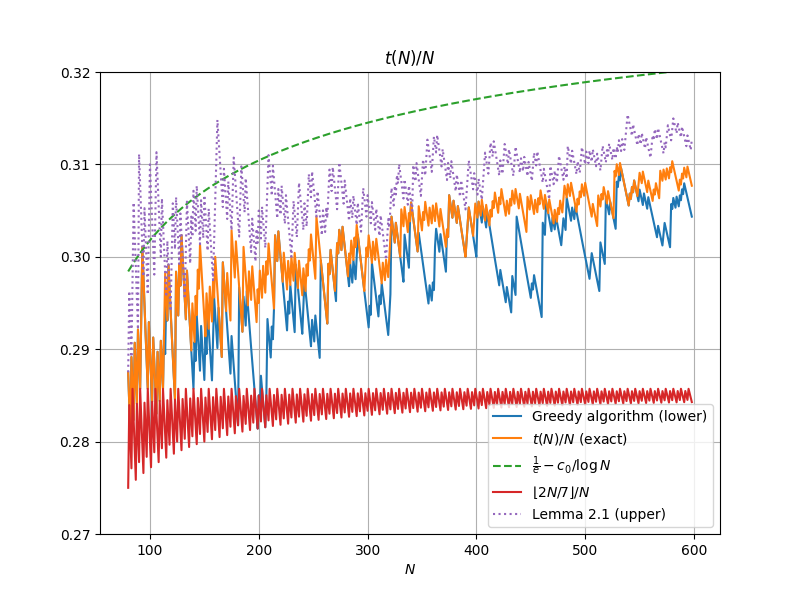
\includegraphics[width=0.8\textwidth]{newplot_600.png}
  \caption{An enlarged version of \Cref{fig1-alt}, displaying the lower bound from the greedy algorithm and the upper bound from \Cref{upper-crit}.  The linear programming upper and lower bounds are exact in this region, except for $N=155$ in which the upper bound is off by one.}\label{fig-zoom}
\end{figure}


We can now prove the upper bound portion of \Cref{main}(iv):

  \begin{proposition}\label{upper-bound}  For large $N$, one has
    $$ \frac{t(N)}{N} \leq \frac{1}{e} - \frac{c_0}{\log N} + O\left( \frac{1}{\log^2 N} \right).$$
    \end{proposition}
    
    \begin{proof}  We apply \Cref{upper-crit} with
      $$ t \coloneqq \frac{1}{e} - \frac{c_0}{\log N} + \frac{C_0}{\log^2 N}$$
    with $C_0$ a large absolute constant to be chosen later.  From Taylor expansion and the Stirling approximation one sees that
    $$ \log N! - N \log t \geq ec_0 \frac{N}{\log N} + (C_0-O(1)) \frac{N}{\log^2 N}$$
    so it will suffice to establish the upper bound
    $$ \sum_{\frac{t}{\lfloor\sqrt{t}\rfloor} < p \leq N} f_{N/t}(p/N) \leq ec_0 \frac{N}{\log N} + O\left( \frac{N}{\log^2 N} \right).$$
    For $N$ large enough, we have $\frac{t}{\lfloor\sqrt{t}\rfloor} \leq \frac{N}{\log N}$, so it suffices to show that
    $$ \sum_{\frac{N}{\log N} \leq p \leq N} f_{N/t}(p/N) \leq ec_0 \frac{N}{\log N} + O\left( \frac{N}{\log^2 N} \right).$$
    On the interval $[1/\log N,1]$, the piecewise smooth function $f_{N/t}$ is bounded by $O(1)$ thanks to \eqref{falpha-bound}, and has a total variation of $O(\log N)$; the same is then true for the rescaled function $x \mapsto f_{N/t}(x/N)$ on $[N/\log N,1]$.  By \Cref{buthe}, \eqref{ecx}, the left-hand side is then
    $$ \int_{N/\log N}^N \left(1-\frac{2}{\sqrt{x}}\right) f_{N/t}(x/N) \frac{dx}{\log x} + O\left( N \exp(-c\sqrt{\log N}) \right)$$
    for some $c>0$.  Discarding the $\frac{2}{\sqrt{x}}$ term, performing a change of variable, and using \eqref{c0-def}, we reduce to showing that
    $$  \int_{1/\log N}^1 f_{N/t}(x) \frac{\log N}{\log(Nx)}\ dx 
    \leq  \int_0^1 f_e(x)\ dx  + O\left( \frac{1}{\log N} \right).$$
    We have the Taylor approximation 
    $$\frac{\log N}{\log(Nx)} = 1 + O\left( \frac{\log(1/x)}{\log N} \right).$$ 
    Applying \eqref{falpha-bound} and the integrability of $\log(1/x)$, we see that the contribution of the error term is acceptable.  Applying a further rescaling by $N/et = 1 + O(1/\log N)$, we reduce to showing that
$$ \int_{N/et\log N}^{N/et} f_{N/t}(Nx/et)\ dx = \int_0^1 f_e(x)\ dx  + O\left( \frac{1}{\log N} \right).$$
But observe that $f_{N/t}(Nx/et) = f_e(x)$ unless $\frac{1}{x}$ is within $O(1/\log N)$ of an integer, which one can calculate to occur on a set of measure $O(1/\log N)$ for $x \in [0,N/et]$.  By \eqref{falpha-bound}, both integrands are bounded by $O(1)$ for all $x \in [0,N/et]$, and the claim follows from the triangle inequality.
\end{proof}
    
We can now establish \Cref{main}(i): 

\begin{proposition}\label{tne} One has $t(N)/N < 1/e$ for $N \neq 1,2,4$.
\end{proposition}

\begin{proof}  From existing data on $t(N)$ (or the linear programming method) one can verify this claim for $N < 80$ (see \Cref{fig1}), so we assume that $N\geq 80$.
  
Applying \Cref{upper-crit}, \eqref{stirling}, it suffices to show that
\begin{equation}\label{base-test-eq}
   \sum_{p \geq \frac{N/e}{\lfloor\sqrt{N/e}\rfloor}} f_{e}(p/N) > \frac{1}{2} \log(2\pi N) + \frac{1}{12N}.
\end{equation}
This may be easily verified numerically in the range $80 \leq N \leq 5000$ (see \Cref{fig2}).
We will discard the $\lfloor\sqrt{N/e}\rfloor$ denominator, and reduce to showing
\begin{equation}\label{test-ineq}
  \sum_{N/e < p \leq N} f_{e}(p/N) > \frac{1}{2} \log(2\pi N) + \frac{1}{12N}
\end{equation}
for $N > 5000$.  On $[1/e,1]$, one can compute
$$ \|f_e\|_{\mathrm{TV}^*(1/e,1]}
= 4 - 2 \log 2$$
so by \Cref{buthe}, \eqref{ecx-2} (noting that $5000 > 1423e$) we have
$$ \sum_{N/e < p \leq N} f_{e}(p/N) \log p
\geq N \int_{1/e}^1 \left(1-\frac{2}{\sqrt{Nx}}\right) f_e(x)\ dx - (4 - 2 \log 2) \tilde E(N).
$$
By upper bounding $\log p$ by $\log N$ and lower bounding $\left(1-\frac{2}{\sqrt{Nx}}\right)$ by $1 - \frac{2}{\sqrt{N/e}}$, it suffices to show that
$$ \left(1 - \frac{2}{\sqrt{N/e}}\right) \int_{1/e}^1 f_e(x)\ dx \geq
(4 - 2 \log 2) \frac{\tilde E(N)}{N}
+ \frac{\log N \log(2\pi N)}{2N} + \frac{\log N}{12N^2},$$
which is easily verified for $N \geq 5000$ (one has $\int_{1/e}^1 f_e(x)\ dx = \frac{2}{e}-\frac{\log 2}{2}=0.3891\dots$ and $4-2\log 2 = 2.613\dots$, while $\tilde E(N)/N \leq 0.015$, and the other two terms on the right-hand side are negligible).
\end{proof}

\begin{figure}
  \centering
  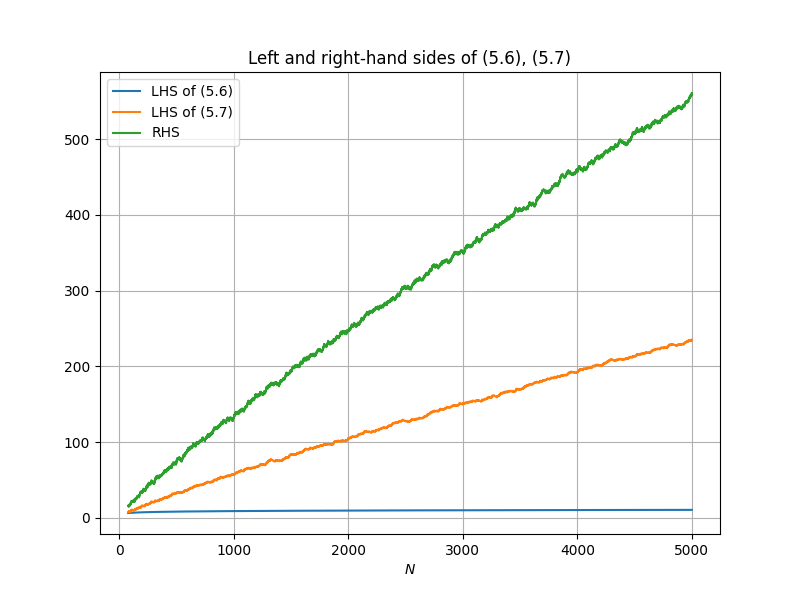
\includegraphics[width=0.8\textwidth]{lhs_rhs.png}
  \caption{A plot of the left and right-hand sides of \eqref{base-test-ineq}, \eqref{test-ineq} for $80 \leq N < 5000$.}\label{fig2}
\end{figure}


\subsection{Modified approximate factorizations}\label{approx-sec}

In this section we present and then analyze an algorithm that, when given parameters $1 \leq t \leq N$, will attempt to construct a $t$-admissible subfactorization $\prod \tuple$ of $N!$ that obeys the criterion in \Cref{t-descrip}.  The algorithm will not always succeed, but when it does, it will certify that $t(N) \geq t$.

The basic idea is to start with an initial approximate factorization $\tuple^{(1)}$ that has small $t$-excess and is close to balance at all small and medium primes, but has no tiny primes, and also has the ``wrong'' selections of large primes.  One then modifies this factorization in a number of ways to return to balance at all non-tiny primes, as well as near-balance at the tiny primes. 

As part of the algorithm, one will often wish to replace a non-$3$-smooth number $x$ with a $3$-smooth upper bound $2^n 3^m$.  A natural choice here would be the least such upper bound $\lceil x \rceil^{\langle 2,3 \rangle}$.  However, this bound may contain an imbalanced number of powers of $2$ and $3$; because $\nu_2(N!) \approx N$ and $\nu_3(N!) \approx N/2$, we would ideally like this $3$-smooth upper bound to have twice as many powers of $2$ as of $3$, that is to say it is a power of $12$.  We therefore introduce the variant quantity
$$ \lceil x \rceil^{\langle 2,3\rangle}_L \coloneqq 12^a \lceil x/12^a \rceil^{\langle 2,3 \rangle}$$
for any real $x \geq L \geq 1$, where $a \coloneqq \lfloor \frac{x/L}{\log 12} \rfloor$ is the largest integer such that $12^a \leq x/L$.  This quantity is $3$-smooth, and has the following bound:

\begin{lemma}[Valuation bounds]\label{val} If $x \geq L \geq 1$ are real numbers, then
$$ x \leq \lceil x \rceil^{\langle 2,3\rangle}_L \leq x e^{\kappa_L}$$
and
$$ \sup_{p_0=2,3} (p_0-1) \nu_{p_0}(\lceil x \rceil^{\langle 2,3\rangle}_L) \leq \frac{2}{\log 12} \log x + \kappa^*_L$$
where
\begin{equation}\label{kappastar-def}
\kappa^*_L \coloneqq (\frac{2}{\log 3} - \frac{2}{\log 12}) \log(12L) + \frac{2}{\log 3} \kappa_L.
\end{equation}
\end{lemma}

This can be compared with the bound
$$ \sup_{p_0=2,3} (p_0-1) \nu_{p_0}(\lceil x \rceil^{\langle 2,3\rangle}) \leq \frac{2}{\log 3} x + \frac{2}{\log 3} \kappa_x$$
that can be obtained from \eqref{kl-def} and the observation that $\log 2 \leq \frac{2}{\log 3}$.  

\begin{proof} The first claim is clear from \eqref{kl-def}, so we focus on the second.  If we write $\lceil x/12^a \rceil^{\langle 2,3 \rangle} = 2^n 3^m$, then by \eqref{kl-def} we have
$$ n \log 2 + m \log 3 \leq \log \frac{x}{12^a} + \kappa_L;$$
since $\log 2 \leq \frac{2}{\log 3}$, this implies that
$$ \max( n, 2m ) \leq \frac{2}{\log 3} \log \frac{x}{12^a}
+ \frac{2}{\log 3} \kappa_L.$$
Hence 
\begin{align*}
  \sup_{p_0=2,3} (p_0-1) \nu_{p_0}(\lceil x \rceil^{\langle 2,3\rangle}) &= \max(2a+n, 2a+2m) \\
  &\leq 2a + \frac{2}{\log 3} \log \frac{x}{12^a}
  + \frac{2}{\log 3} \kappa_L \\
  &= \frac{2}{\log 12} \log x + 
  \left(\frac{2}{\log 3} - \frac{2}{\log 12}\right) \log \frac{x}{12^a}
  + \frac{2}{\log 3} \kappa_L \\
  \frac{2}{\log 12} \log x + 
  \left(\frac{2}{\log 3} - \frac{2}{\log 12}\right) \log(12L)
  + \frac{2}{\log 3} \kappa_L,
\end{align*}
giving the claim.
\end{proof}

\subsection{Description of algorithm}\label{alg-desc}

In addition to the given parameters $1 \leq t \leq N$, we require additional natural number parameters $A,K$ and a real parameter $L \geq 1$ obeying the hypotheses
\begin{equation}\label{condition}
  9L, K^2 (1+\sigma) < t; \quad K\sqrt{N} < t; \quad \sigma < 1; \quad K \geq L \geq 4.5; 
\end{equation}
where
\begin{equation}\label{sigma-def}
  \sigma \coloneqq \frac{3N/t}{A}.
\end{equation}  
There is some freedom to select parameters here, but roughly speaking one would like to have $1 \lll A \lll K \lll \sqrt{t}$.

It will be convenient to divide the set of primes into the following ranges:
\begin{itemize}
\item \emph{Tiny primes} $p=2,3$.
\item \emph{Small primes} $3 < p \leq K$.
\item \emph{Borderline small primes} $K < p \leq K(1+\sigma)$.
\item \emph{Medium primes} $K(1+\sigma) < p \leq t/K$.
\item \emph{Large primes} $p > t/K$.
\end{itemize}

With such parameters in hand, we can consider the following algorithm.


\begin{enumerate}
\item[(1)] Let $I$ denote the elements of the interval\footnote{Numerically, it would be slightly better to use the closed interval $[t,t(1+\sigma)]$ instead of the half-open interval $(t,t(1+\sigma)]$, but we will consistently aim to use half-open intervals here to be compatible with standard notation for the prime counting function $\pi(x)$.} $(t,t(1+\sigma)]$ that are coprime to $6$.  Let $\tuple^{(1)}$ be the elements of $I$, each occurring with multiplicity $A$.  This multiset is $t$-admissible, and $\prod \tuple^{(1)}$ is not divisible by tiny primes $2,3$.  (It will have approximately the right number of primes for small, borderline, and medium $3 < p \leq t/K$, though it may have quite different prime factorization at large primes $p>t/K$.)
\item[(2)] Remove any element from $\tuple^{(1)}$ that contains a large prime factor $p > t/K$, and call this new multiset $\tuple^{(2)}$.  It remains $t$-admissible with no tiny prime factors, though it tends to acquire a $p$-surplus at small primes $3 < p \leq K$.
\item[(3)] For each $p > t/K$, add in $\nu_p(N!)$ copies of the number $p \lceil t/p \rceil$ to $\tuple^{(2)}$, and call this new multiset $\tuple^{(3)}$.   Now $\tuple^{(3)}$ is $t$-admissible and in balance at all large primes $p>t/K$, but will expected to enjoy some surplus at small and borderline primes $3 < p \leq K(1+\sigma)$, and be in balance for medium priems $K(1+\sigma) < p \leq t/K$.  (It will now also contain a few tiny prime factors, but will generally still have a large surplus at those primes.)
\item [(4)] For small primes $3 < p \leq K$ at which there is a surplus $\nu_p(\N!/\prod \tuple) > 0$, multiply all these primes together, and use the greedy algorithm to group them into factors $x_1, \dots, x_M$ in the range
$(t/K^2, t/K]$, together with possibly one exceptional factor $x_*$ in the range $(1, t/K]$.  For each of these factors $x_i$ or $x_*$, add the quantity $x_i \lceil t/x_i \rceil^{\langle 2,3 \rangle}_{4.5}$ or $x_* \lceil t/x_* \rceil^{\langle 2,3 \rangle}_{4.5}$ to $\tuple^{(3)}$, and call this new multiset $\tuple^{(4)}$.  We apply the same procedure for borderline or medium primes $K < p \leq t/K$, but without the initial grouping procedure. Thus $\tuple^{(4)}$ has no surplus at small, borderline, or medium primes $3 < p \leq t/K$ (and is still $t$-admissible and in balance for $p>t/K$).
\item[(5)] For each small, borderline, or medium prime $3 < p \leq t/K$ at which there is a deficit $\nu_p(\prod \tuple/N!) > 0$, replace $\nu_p(\prod \tuple/N!)$ copies of $p$ in the prime factorizations of elements of $\tuple^{(4)}$ with $\lceil p \rceil^{\langle 2,3 \rangle}_{4.5}$ instead, and call this new multiset $\tuple^{(5)}$.  
\item[(6)] By construction, $\tuple^{(5)}$ is $t$-admissible and will be in balance at all non-tiny primes $p>3$, and is thus $N!/\prod \tuple^{(5)}$ is of the form $2^n 3^m$ for some integers $n,m$.  Let $2^{n_0}, 3^{m_0}$ be the largest powers of $2$ and $3$ respectively less than or equal to $t/L$, and set $2^{n_1} 3^{m_1} \coloneqq \lceil t/2^{n_0} \rceil^{\langle 2,3 \rangle}$ and $2^{n_2} 3^{m_2} \coloneqq \lceil t/2^{n_0} \rceil^{\langle 2,3 \rangle}$.  If one cannot express $(n,m)$ as a positive linear combination $\alpha_1 (n_1,m_1) + \alpha_2 (n_2,m_2)$ of $(n_1,m_1)$ and $(n_2,m_2)$, \texttt{HALT} with an error.  Otherwise, add $\lfloor \alpha_1 \rfloor$ copies of $2^{n_1} 3^{m_1}$ and $\lfloor \alpha_2 \rfloor$ copies of $2^{n_2} 3^{m_2}$ to $\tuple^{(5)}$, and call this tuple $\tuple^{(6)}$.  (This will largely eliminate the surplus at $2$ and $3$.)
\item[(7)] If the criterion in \Cref{t-descrip} is obeyed by $\tuple^{(6)}$, then we have successfully established\footnote{If desired, one could implement the proof of \Cref{t-descrip} as a final component of this algorithm, that is to say one removes elements from $\tuple^{(6)}$ to make the cardinality exactly $N$, and then distributes any surplus primes arbitrarily to create a $t$-admissible factorization of $N!$ of cardinality exactly $N$.} that $t(N) \geq t$.  Otherwise, \texttt{HALT} the algorithm with an error. 
\end{enumerate}

The expected $p$-surpluses or $p$-deficits at various stages of this process are summarized in \Cref{algorithm-table}.

\begin{table}[ht]
  \centering
  \begin{tabular}{|c|c|c|c|c|c|}
  \hline
   & Tiny $p$ & Small $p$ & Borderline $p$ & Medium $p$ & Large $p$ \\
  \hline
  $\tuple^{(1)}$ & Max. surplus & Near balance & Near balance & Near balance & ??? \\
  $\tuple^{(2)}$ & Max. surplus & Med. surplus & Med. surplus? & Near balance & Max. surplus \\
  $\tuple^{(3)}$ & Lg. surplus & Sm. surplus? & Med. surplus? & Near balance & Balance \\
  $\tuple^{(4)}$ & Lg. surplus & Balance? & Balance?
 & Balance/sm. deficit & Balance \\
  $\tuple^{(5)}$ & Lg. surplus & Balance & Balance & Balance  & Balance \\
  $\tuple^{(6)}$ & Sm. surplus & Balance & Balance & Balance  & Balance \\
  $\tuple^{(7)}$ & Balance & Balance & Balance & Balance  & Balance \\ 
  \hline
  \end{tabular}
  \caption{Evolution of the surpluses and deficits of the multisets $\tuple^{(i)}$, $i=1,\dots,6$; we describe the size of these surpluses and deficits informally as ``small'', ``medium'', ``large'', or ``maximal''.  For entries with a question mark, we allow the possibility of a tiny deficit.  For the entry marked ???, all behavior from large surpluses to large deficits are possible. The final step $\tuple^{(7)}$ is an optional one, if one wishes to convert the subfactorization $\tuple^{(6)}$ to an exact factorization.}\label{algorithm-table}
  \end{table}
  

\subsection{Analysis of Step 7}

We now analyze the above algorithm, starting from the final Step 7 and working backwards to Step 1, to establish sufficient conditions for the algorithm to successfully demonstrate that $t(N) \geq t$.

It will be convenient to introduce the following notation.
For $a_+,a_- \in [0,+\infty]$, we define the asymmetric norm $|x|_{a_+,a_-}$ of a real number $x$ by the formula
$$ 
|x|_{a_+,a_-} \coloneqq  \begin{cases} 
  a_+ |x| & x\geq 0 \\
  a_- |x| & x\leq 0,
\end{cases}
$$
with the usual convention $+\infty \times 0 = 0$.
If $a_+,a_-$ are finite, this function is Lipschitz with constant $\max(a_+,a_-)$.  One can think of $a_+$ as the ``cost'' of making $x$ positive, and $a_-$ as the
``cost'' of making $x$ negative. We can then rewrite the termination condition of \Cref{t-descrip} (using the fact that $\tuple^{(6)}$ is a subfactorization of $N!$) as
$$
\excess_t(\tuple^{(6)}) + \sum_p \left| \nu_p\left(\frac{N!}{\prod \tuple^{(6)}}\right) \right|_{\log p,\infty}
\leq \log N! - N \log t.$$
If we assume that $t = N/e^{1+\delta}$ for some $\delta > 0$, we can use the Stirling approximation \eqref{stirling} to reduce to the sufficient condition
$$
\excess_t(\tuple^{(6)}) + \sum_p \left| \nu_p\left(\frac{N!}{\prod \tuple^{(6)}}\right) \right|_{\log p,\infty}
\leq \delta N + \log \sqrt{2\pi N}
$$
which we choose to normalize as
\begin{equation}\label{step7-cond}
\frac{1}{N}  \excess_t(\tuple^{(6)}) + \frac{1}{N} \sum_p \left| \nu_p\left(\frac{N!}{\prod \tuple^{(6)}}\right) \right|_{\log p,\infty}
  \leq \delta + \frac{\log \sqrt{2\pi N}}{N}.
\end{equation}


\subsection{Analysis of Step 6}

Now we analyze Step 6, using the quantity $\kappa_L$ introduced in \eqref{kappa-def}.  The main tool we need is the following efficient subfactorization of $3$-smooth numbers.

{\bf TODO: draw picture of $n_0$, $m_0$, etc.}

\begin{lemma}[Efficient subfactorization of $3$-smooth numbers]\label{bound23}  Let $L \geq 1$.  Let $t > 3L$ and let $2^n 3^m$ be a $3$-smooth number with $n,m$ positive and obeying the condition
  \begin{equation}\label{B-bound}
    \frac{\log(3L)+\kappa_L}{\log t - \log(3L)} \leq \frac{n \log 2}{m \log 3} \leq \frac{\log t - \log(2L)}{\log(2L)+\kappa_L}.
  \end{equation}
    Then one can find a $t$-admissible subfactorization $\tuple$ of $2^n 3^m$ such that
  \begin{equation}\label{excess-bound} 
    \excess_t(\tuple) \leq \kappa_L \frac{n \log 2 + m \log 3}{\log t} 
  \end{equation}
  and
  \begin{equation}\label{surplus-bound} 
    \sum_{p_0=2,3} |\nu_{p_0}(2^n 3^m/\tuple)|_{\log p_0,\infty} \leq 2(\log t + \kappa_L).
  \end{equation}
  \end{lemma}
  
  In practice, $\log t$ will be significantly larger than $\log(2L)$ or $\log(3L)$, and so the hypothesis \eqref{B-bound} will be relatively mild, as long as $n$ and $m$ are both reasonably large.
  
  \begin{proof}  Let $2^{n_0}, 3^{m_0}$ be the largest powers of $2$ and $3$ less than or equal to $t/L$ respectively, thus
  \begin{equation}\label{L1}
   L \leq \frac{t}{2^{n_0}} < 2L
  \end{equation}
    and
    \begin{equation}\label{L2}  L \leq \frac{t}{3^{m_0}} < 3L. \end{equation}
  From \eqref{kappa-def}, the $3$-smooth numbers $2^{n_1} 3^{m_1} \coloneqq \lceil t/2^{n_0} \rceil^{\langle 2,3 \rangle}$, $2^{n_2} 3^{m_2} \coloneqq \lceil t/3^{m_0} \rceil^{\langle 2,3 \rangle}$ obey the estimates
  \begin{equation}\label{ab} 
    \frac{t}{2^{n_0}} \leq 2^{n_1} 3^{m_1} \leq e^{\kappa_L} \frac{t}{2^{n_0}}
  \end{equation}
  and
  \begin{equation}\label{ab-2}
   \frac{t}{3^{m_0}} \leq 2^{n_2} 3^{m_2} \leq e^{\kappa_L} \frac{t}{3^{m_0}},
  \end{equation}
  or equivalently
  \begin{equation}\label{ab-equiv} 
    t \leq 2^{n_0+n_1} 3^{m_1}, 2^{n_2} 3^{m_0+m_2} \leq e^{\kappa_L} t.
  \end{equation}
  We can use \eqref{L1}, \eqref{ab} to bound
  \begin{align*}
    \frac{n_0 + n_1}{m_1} &\geq \frac{n_0}{\log (e^{\kappa_L} \frac{t}{2^{n_0}}) / \log 3} \\
    &\geq \frac{(\log t - \log(2L)) / \log 2}{ (\log(2L)+\kappa_L) / \log 3 }
  \end{align*}
  (with the convention that this bound is vacuously true for $m_1=0$). Similarly, from \eqref{L2}, \eqref{ab-2} we have
  \begin{align*}
    \frac{n_2}{m_0+m_2} &\leq \frac{\log(e^\kappa \frac{t}{3^{m_0}}) / \log 2}{m_0} \\
    &\leq \frac{(\log(3L)+\kappa)/\log 2}{(\log t-\log(3L))/\log 3}
  \end{align*}
  and hence by \eqref{B-bound}
  \begin{equation}\label{m-wedge} \frac{n_2}{m_0+m_2} \leq \frac{n}{m} \leq \frac{n_0+n_1}{m_1}.
  \end{equation}
  Thus we can write $(n,m)$ as a non-negative linear combination
  $$ (n,m) = \alpha_1 (n_0+n_1,m_1) + \alpha_2 (n_2,m_0+m_2)$$
  for some real $\alpha_1, \alpha_2 \geq 0$. We now take our subfactorization $\tuple$ to consist of $\lfloor \alpha_1 \rfloor$ copies of the $3$-smooth number $2^{n_0+n_1} 3^{m_1}$ and $\lfloor \alpha_2 \rfloor$ copies of the $3$-smooth number $2^{n_2} 3^{m_0+m_2}$.  By \eqref{ab-equiv}, each term $2^{n'} 3^{m'}$ here is admissible and contributes a $t$-excess of at most $\kappa_L$, which is in turn bounded by $\kappa_L \frac{n' \log 2 + m' \log 3}{\log t} $.  Adding these bounds together, we obtain \eqref{excess-bound}.
  
  As a subfactorization of $2^n 3^m$, the multiset $\tuple$ has a $2$-surplus of at most $n_0+n_1+n_2$ and a $3$-surplus of at most $m_0+m_2+m_1$, hence
  $$ \sum_{p_0=2,3} \nu_{p_0}\left(\frac{2^n 3^m}{\prod \tuple}\right) \log p_0 \leq \log 2^{n_0+n_1} 3^{m_1} + \log 2^{n_2} 3^{m_0+m_2},$$
  and the bound \eqref{surplus-bound} follows from \eqref{ab-equiv}.
  \end{proof}
  
We now use this lemma to analyze Step 6 as follows.

\begin{proposition}\label{step6-reduce} Let $L \geq 1$.
  Let $3L < t = N/e^{1+\delta}$ for some $\delta>0$, and let $1 \leq K \leq t$ and $A \geq 1$.  Suppose that the algorithm in \Cref{alg-desc} with the indicated parameters reaches the end of Step 5 with a multiset $\tuple^{(5)}$ obeying the following hypotheses:
\begin{itemize}
  \item[(i)] (Small excess and surplus at non-tiny primes)
  \begin{equation}\label{new-balance-3}
  \begin{split}
    &\frac{1}{N} \excess_t(\tuple^{(5)}) + \frac{1}{N} \sum_{p>3} \left|\nu_p\left(\frac{N!}{\prod \tuple^{(5)}}\right)\right|_{\log p,\infty}  \\
    &\quad + \frac{\kappa_L \log \sqrt{12}}{\log t} + \frac{3}{2} \frac{\log N}{N} \leq \delta + \frac{\log \sqrt{2\pi}}{N}.
  \end{split}
  \end{equation}
  \item[(ii)] (Large surpluses at tiny primes) One has
\begin{equation}\label{qn} 
\frac{1}{N} \max_{p_0=2,3} (p_0-1) \nu_{p_0}\left(\prod \tuple^{(5)}\right) < 1-\alpha
\end{equation}
where 
\begin{equation}\label{qntl} 
  \begin{split}
\alpha &\coloneqq \max(\alpha_1,\alpha_2) \\
\alpha_1 &\coloneqq \frac{\log(3L)+\kappa_L}{\log t - \log(3L)} \frac{\log 3}{2 \log 2} + \frac{\log N}{N \log 2} + \frac{1}{N} \\
\alpha_2 &\coloneqq \frac{\log(2L)+\kappa_L}{\log t - \log(2L)} \frac{2\log 2}{\log 3} + \frac{2\log N}{N \log 3} + \frac{2}{N}.
  \end{split}
\end{equation}
\end{itemize}
Then $t(N) \geq t$.
\end{proposition}

\begin{proof} Write $n \coloneqq \nu_2(N!/\prod \tuple^{(5)})$ and $m \coloneqq \nu_3(N!/\prod \tuple^{(5)})$.  From \eqref{legendre} we have $n \leq N$ and $m \leq N/2$, hence
$$ n \log 2 + m \log 3 \leq N \log \sqrt{12}.$$
  From \eqref{qn}, \eqref{qntl}, \eqref{legendre} we have
\begin{align*}
  n &= \nu_2(N!) - \nu_2\left(\prod \tuple^{(5)}\right) \\
  &> N - (1+\log N/\log 2) - (1-\alpha_1) N \\
  &\geq \frac{\log(3L) + \kappa_L}{\log t - \log(3L)} \frac{N \log 3}{2\log 2} \\
  &\geq \frac{\log(3L) + \kappa_L}{\log t - \log(3L)} \frac{m \log 3}{\log 2}  
\end{align*}  
and similarly
\begin{align*}
  m &= \nu_3(N!) - \nu_3\left(\prod \tuple^{(5)}\right) \\
  &> \frac{N}{2} - (1+\log N/\log 3) - (1-\alpha_2) \frac{N}{2} \\
  &\geq \frac{\log(2L) + \kappa_L}{\log t - \log(2L)} \frac{N \log 2}{\log 3} \\
  &\geq \frac{\log(3L) + \kappa_L}{\log t - \log(3L)} \frac{n \log 2}{\log 3}.  
\end{align*}  
In particular, $n,m$ are positive and the condition \eqref{B-bound} holds.  Applying \Cref{bound23}, we can find a subfactorization $\tuple'$ of $2^n 3^m$ with an excess of at most $(\kappa_L \log \sqrt{12}) \frac{N}{\log t}$, and with
  $$ \sum_{p_0=2,3} \left|\nu_{p_0}\left(\frac{2^n 3^m}{\prod \tuple'}\right)\right|_{\log p_0,\infty}
   \leq 2(\log t + \kappa_L) \leq 2 \log N$$
   where we have used \eqref{kl-triv} and the fact that $\log t\leq \log N-1$.    Then $\tuple^{(6)} = \tuple^{(5)} \cup \tuple'$ is another $t$-admissible multiset, and from \eqref{new-balance-3}, we obtain the previous sufficient condition  \eqref{step7-cond}.
  \end{proof}
  
\subsection{Analysis of Step 5}

We can use the surplus tiny primes to efficiently deal with larger surplus primes, as follows.

\begin{proposition}\label{balance-23'}  Let $1 \leq K \leq t \leq N$, $A \geq 1$, and $L \geq 1$ be parameters such that $9L < t = N/e^{1+\delta}$ for some $\delta>0$, and \eqref{condition} holds.  Suppose that the algorithm in \Cref{alg-desc} with the indicated parameters reaches the end of Step 4 to produce a multiset $\tuple^{(4)}$ such that the quantities
  \begin{align}
    Y_1 &\coloneqq \frac{1}{N} \sum_{3 < p \leq K} \left|\nu_p\left(\frac{N!}{\prod \tuple^{(3)}}\right)\right|_{\frac{\log p}{\log (t/K^2)},\infty}  \label{y1-def}\\
    Y_2 &\coloneqq \frac{1}{N} \sum_{K < p \leq t/K} \left|\nu_p\left(\frac{N!}{\prod \tuple^{(3)}}\right)\right|_{1,\infty}\label{y2-def}
  \end{align}
  obeying the bounds
\begin{equation}\label{new-balance-4}
  \begin{split}
&    \frac{1}{N}  \excess_t(\tuple^{(4)}) + \kappa_{4.5} (Y_1 + Y_2) 
 \\
&\quad  + \frac{\kappa_L \log \sqrt{12}}{\log t}  + \frac{3}{2} \frac{\log N}{N}   \leq \delta. 
  \end{split}
 \end{equation}
and
 \begin{align*}
  &\frac{1}{N} \sup_{p_0=2,3} (p_0-1) \nu_{p_0}\left(\prod \tuple^{(4)}\right) + \frac{2}{\log 12} (\log(K^2)+\kappa^*_{4.5}) Y_1 + \frac{2}{\log 12} (\log(t/K)+\kappa^*_{4.5}) (Y_2+\frac{1}{N}) \\
&\quad
  \leq 1 - \alpha.
 \end{align*}
Then $t(N) \geq t$.
\end{proposition}

\begin{proof} By \eqref{new-balance-4}, $\tuple^{(4)}$ is a subfactorization of $N!$, and by construction it is in balance at all large primes $p>t/K$. Consider all the $p$-surplus small primes $3 < p \leq K$, thus each such prime is considered with multiplicity $\nu_p(N!/\prod \tuple^{(4)})$.  
Using the greedy algorithm, one can factor the product of all these primes into $M$ factors $c_1,\dots,c_M$ in the interval $(t/K^2, t/K]$ for some $M$, times at most one exceptional factor $c_*$ in $(1,t/K^2]$.  We have the bound
$$ \left(\frac{t}{K^2}\right)^{M'} \leq
\prod_{3 < p \leq K} \nu_p\left(\frac{N!}{\prod \tuple^{(4)}}\right)$$
and hence on taking logarithms and using \eqref{y1-def} we have
$$
M \leq NY_1. 
$$
Also, the number of borderline or medium primes $K < p \leq t/K$ appearing in $N!/\prod \tuple^{(4)}$, counting multiplicity, is $NY_2$.

For each of the $M$ factors $c_i$, we introduce the $3$-smooth number $\lceil t/c_i\rceil^{\langle 2,3\rangle}_{4.5} = 2^{n_i} 3^{m_i}$, which by \Cref{val} lies in the interval $[t/c_i,e^{\kappa_{4.5}} t/c_i]$; similarly, for the exceptional factor $c_*$ we introduce a $3$-smooth number $\lceil t/c_* \rceil^{\langle 2,3 \rangle}_{4.5} = 2^{n_*} 3^{m_*}$ in the interval $[t/c_*,e^{\kappa_{4.5}} t/c_*]$.  Finally, for the $Y_2$ borderline or medium primes $K < p \leq t/K$ discussed above, we introduce the $3$-smooth number $\lceil t/p\rceil^{\langle 2,3\rangle}_{4.5} = 2^{n'_p} 3^{m'_p}$, which lies in the interval $[t/p,e^{\kappa_{4.5}} t/p]$.  We adjoin the $3$-smooth numbers $\lceil t/c_i\rceil^{\langle 2,3\rangle}_{4.5} c_i = 2^{n_i} 3^{m_i} c_i$ for $i=1,\dots,M$ as well $\lceil t/c_*\rceil^{\langle 2,3\rangle}_{4.5} c_* = 2^{n_*} 3^{m_*} c_*$ and $\lceil t/p \rceil^{\langle 2,3\rangle}_{4.5} p = 2^{n'_p} 3^{m'_p} c_p$ to the $t$-admissible multiset $\tuple^{(4)}$ to create a new $t$-admissible multiset $\tuple^{(5)}$.  

For each $i=1,\dots,M$, we have from \Cref{val} that
$$ \max( n_i, 2m_i ) \leq \frac{2}{\log 12} (\log K^2 + \kappa^*_{4.5}).$$
Similarly we have
$$ \max( n_*, 2m_* ) \leq \frac{2}{\log 12} (\log (t/K) + \kappa^*_{4.5})$$
and
$$ \max( n'_p, 2m'_p ) \leq \frac{2}{\log 12} (\log (t/K) + \kappa^*_{4.5})$$
for the medium primes $m$.
Hence
\begin{align*} 
  & \sup_{p_0=2,3} (p-1) \nu_{p_0}\left(\prod \tuple^{(5)}\right) \\
  &\quad \leq \sup_{p_0=2,3} (p-1) \nu_{p_0}\left(\prod \tuple^{(4)}\right) \log p_0 \\
  &\quad + \frac{2}{\log 12} NY_1 (\log K^2 + \kappa^*_{4.5}) + \frac{2}{\log 12} (NY_2+1) (\log(t/K) + \kappa^*_{4.5}).
\end{align*}
Each of the new factors in $\tuple^{(5)}$ contributes an excess of at most $\kappa_L$, so that
$$ \excess_t(\tuple^{(5)})  \leq \excess_t(\tuple^{(4)}) + \kappa_L (NY_1+NY_2+1).$$
We conclude that $\tuple^{(5)}$ obeys the hypotheses of \Cref{step6-reduce} (using \eqref{kl-triv} to bound $\kappa_L$ by $\log\sqrt{2\pi}$ to clean up some lower order terms), and the claim follows.
\end{proof}

\subsection{Analysis of Step 4}

The surplus tiny primes can also be used to deal with any larger primes that are in deficit, as follows.

\begin{proposition}\label{step4-reduce}  Let $L \geq 1$.  Let $9L < t = N/e^{1+\delta}$ for some $\delta>0$ be such that \eqref{condition} holds, and suppose that the algorithm reaches the end of Step 3 to produce a multiset $\tuple^{(3)}$ such that the quantities
  \begin{align}
    Y_1^+ &\coloneqq \frac{1}{N} \sum_{3 < p \leq K} \left|\nu_p\left(\frac{N!}{\prod \tuple^{(3)}}\right)\right|_{\frac{\log p}{\log (t/K^2)},0}  \label{y1p-def}\\
    Y_1^- &\coloneqq \frac{1}{N} \sum_{3 < p \leq K} \left|\nu_p\left(\frac{N!}{\prod \tuple^{(3)}}\right)\right|_{0,1}.\label{y1m-def} \\
    Y^\pm_2 &\coloneqq \frac{1}{N} \sum_{K < p \leq t/K} \left|\nu_p\left(\frac{N!}{\prod \tuple^{(3)}}\right)\right|\label{y2pm-def}
  \end{align}
    obey the hypotheses
\begin{equation}\label{new-balance-5}
    \begin{split}
&     \frac{1}{N} \excess_t(\tuple^{(3)}) + \kappa_{4.5} (Y_1^+ + Y_1^- + Y_\pm)\\
&\quad + \frac{\kappa_L \log \sqrt{12}}{\log t} + \frac{3}{2} \frac{\log N}{N}  \leq \delta.
    \end{split}
  \end{equation}
and
  \begin{equation}\label{nstarb}
    \begin{split}
&\frac{1}{N} \sup_{p_0=2,3} (p-1) \nu_{p_0}\left(\prod \tuple^{(3)}\right) \\
&\quad + \frac{2}{\log 12} (\log K^2 +\kappa^*_{4.5}) Y_1^+ + \frac{2}{\log 12} (\log K + \kappa^*_{4.5}) Y_1^- + \frac{2}{\log 12} (\log(t/K) +\kappa^*_{4.5}) (Y_2^\pm+\frac{1}{N})  
\\
  &\quad  \leq 1-\alpha
  \end{split}
\end{equation}
     Then $t(N) \geq t$.
\end{proposition}

\begin{proof} Suppose there is a non-tiny prime $p>3$ with a positive $p$-deficit
$|\nu_p(N!/\prod \tuple^{(3)})|_{0,1} > 0$.  Since $\tuple^{(3)}$ is in balance at all large primes, we have $3 < p \leq t/K$.  We locate an element of $\tuple^{(3)}$ that contains $p$ as a factor, and replaces it with $\lceil p \rceil^{\langle 2,3 \rangle}_{4.5} = 2^{n_p} 3^{m_p}$, which increases that factor by at most $\exp(\kappa_{4.5})$ thanks to \Cref{val}.  This procedure reduces the $p$-deficit by one, adds at most $\kappa_{4.5}$ to the $t$-excess, and increments $\sup_{p_0=2,3} (p_0-1)\nu_{p_0}(N!/\prod \tuple^{(3)})$ by  at most $\frac{2}{\log 12}(\log(t/K) + \kappa^*_{4.5})$, thanks to \Cref{val}.
So if we apply this procedure to clear all deficits at non-tiny primes, the resulting multiset $\tuple^{(4)}$ has a $t$-excess of
$$ \excess_t(\tuple^{(4)}) \leq \excess_t(\tuple^{(3)})  + \sum_{p > 3} \left|\nu_p\left(\frac{N!}{\prod \tuple^{(3)}}\right)\right|_{0,\kappa_{4.5}}$$
and hence
\begin{align*}
  &\frac{1}{N} \excess_t(\tuple^{(4)}) + \kappa_{4.5} (Y_1 + Y_2) \\
&\leq \frac{1}{N} \excess_t(\tuple^{(4)}) +
\kappa_{4.5} (Y^+_1 + Y^-_1 + Y_2^\pm).
\end{align*}
Similarly we have
$$\sup_{p_0=2,3} (p_0-1) \nu_{p_0}\left(\prod \tuple^{(4)}\right)  \leq
\sum_{p_0=2,3} (p_0-1) \nu_{p_0}\left(\prod \tuple^{(3)}\right) + \frac{2}{\log 12} \sum_{p>3} \left|\nu_p\left(\frac{N!}{\prod \tuple^{(3)}}\right)\right|_{0, \log(t/K)+\kappa^*_{4.5}}$$
and hence
\begin{align*}
  &\frac{1}{N} \sup_{p_0=2,3} (p_0-1) \nu_{p_0}\left(\prod \tuple^{(4)}\right) + \frac{2}{\log 12} (\log(K^2)+\kappa^*_{4.5}) Y_1 + \frac{2}{\log 12} (\log(t/K)+\kappa^*_{4.5}) (Y_2+\frac{1}{N}) \\
  &\quad \leq 
  \frac{1}{N} \sup_{p_0=2,3} (p_0-1) \nu_{p_0}\left(\prod \tuple^{(3)}\right)+ \frac{2}{\log 12}  (\log(K^2)+\kappa^*_{4.5}) Y^+_1 \\
  &\quad \quad + \frac{2}{\log 12} (\log K + \kappa^*_{4.5}) Y^-_1 + \frac{2}{\log 12} (\log(t/K)+\kappa^*_{4.5}) (Y^\pm_2+\frac{1}{N}).
\end{align*}
The hypotheses of \Cref{balance-23'} are now satisfied, and we are done.
\end{proof}

\subsection{Analysis of Step 3}

From direct inspection of Step 3, we see that  borderline or medium primes $K < p \leq t/K$ are unaffected by this step:
\begin{equation}\label{step3-unaffected}
  \nu_p\left(\frac{N!}{\prod \tuple^{(3)}}\right) = \nu_p\left(\frac{N!}{\prod \tuple^{(2)}}\right).
\end{equation}
For tiny or small primes $p_1 \leq K$, we instead have
$$
\nu_{p_1}\left(\frac{N!}{\prod \tuple^{(3)}}\right) = \nu_{p_1}\left(\frac{N!}{\prod \tuple^{(2)}}\right) - \sum_{p > t/K} \nu_p(N!) \nu_{p_1}( \lceil t/p \rceil ).$$
From \eqref{condition} we see that all large primes $p>t/K$ are larger than $\sqrt{N}$, hence by \eqref{legendre} $\nu_p(N!) = \lfloor N/p\rfloor$.  Meanwhile, $\lceil t/p \rceil$ is at most $K$.  Thus, making the change of variables $m \coloneqq \lceil t/p \rceil$, we can also write
\begin{equation}\label{step3-affected}
\nu_{p_1}\left(\frac{N!}{\prod \tuple^{(3)}}\right) = \nu_{p_1}\left(\frac{N!}{\prod \tuple^{(2)}}\right) - \sum_{m \leq K} \nu_{p_1}(m) \sum_{\frac{t}{m} \leq p < \frac{t}{m-1}} \lfloor \frac{N}{p} \rfloor.
\end{equation}
Finally, the $t$-excess after Step 3 can be computed as
$$
\excess_t(\tuple^{(3)}) = 
\excess_t(\tuple^{(2)}) + \sum_{t/K < p \leq N} \nu_p(N!) \log \frac{p \lceil t/p \rceil}{t}$$
and hence by \eqref{legendre} and \eqref{falpha-def}
$$
\excess_t(\tuple^{(3)}) = 
\excess_t(\tuple^{(2)}) + \sum_{t/K < p \leq N} f_{N/t}(p/N).$$
If we bound $f_{N/t}(p/N)$ by $\frac{1}{\log(t/K)} f_{N/t}(p/N) \log p$ and apply \Cref{buthe}, we conclude
\begin{equation}\label{step3-excess}
\frac{1}{N} \excess_t(\tuple^{(3)}) \leq 
 \frac{1}{N}\excess_t(\tuple^{(2)}) + \frac{1}{\log(t/K)} \int_{t/NK}^1 f_{N/t}(x)\ dx + \|f_{N/t}\|_{\mathrm{TV}^*((t/NK,1])} \frac{E(N)}{N \log(t/K)}.  
\end{equation}


\subsection{Analysis of Step 2}

Step 2 removes $A$ copies of every factor of the form $mp$ when $p > t/K$ and $mp \in I$, which forces $m$ coprime to $6$ and $m \leq K(1+\sigma)$.  Thus this procedure does not affect medium primes $K(1+\sigma) < p \leq t/K$:
\begin{equation}\label{step2-unaffected}
  \nu_p\left(\frac{N!}{\prod \tuple^{(2)}}\right) = \nu_p\left(\frac{N!}{\prod \tuple^{(1)}}\right).
\end{equation}
It also does not generate any tiny primes $p_0=2,3$, thus:
\begin{equation}\label{step2-tiny}
\sum_{p_0=2,3}  \nu_{p_0}\left(\frac{N!}{\prod \tuple^{(2)}}\right) \log p_0 = 0.
\end{equation}
For borderline primes $K < p_1 \leq K(1+\sigma)$, this step removes $A$ copies of $p_1 p$ whenever $p_1 p \in I$ and $p \geq t/K$, adding to the $p_1$-surplus $p_1$, but otherwise does not affect this surplus; thus
\begin{equation}\label{step2-borderline}
  \nu_{p_1}\left(\frac{N!}{\prod \tuple^{(2)}}\right) = \nu_{p_1}\left(\frac{N!}{\prod \tuple^{(1)}}\right) +
  A \left(\pi\left(\frac{t(1+\sigma)}{p_1}\right) + \pi\left(\frac{t}{K}\right)\right).
\end{equation}
For small primes $3 < p_1 \leq K$, we instead have
$$
  \nu_{p_1}\left(\frac{N!}{\prod \tuple^{(2)}}\right) = \nu_{p_1}\left(\frac{N!}{\prod \tuple^{(1)}}\right) +
  A \sum_{m \leq K(1+\sigma)}^* \nu_{p_1}(m) \left(\pi\left(\frac{t(1+\sigma)}{m}\right) - \pi\left(\frac{t}{\min(K,m)}\right)\right),
$$
where the notation $\sum^*$ indicates that the summation variable $m$ is required to be coprime to $6$.  We can split this as
\begin{equation}\label{step2-small}
  \nu_{p_1}\left(\frac{N!}{\prod \tuple^{(2)}}\right) = \nu_{p_1}\left(\frac{N!}{\prod \tuple^{(1)}}\right) +
  A \sum_{m \leq K}^* \nu_{p_1}(m) \left(\pi\left(\frac{t(1+\sigma)}{m}\right) - \pi\left(\frac{t}{m}\right)\right) + N Z_{p_1}
\end{equation}
where
\begin{equation}\label{zp-def}
   Z_{p_1} \coloneqq 
\frac{A}{N} \sum_{K < m \leq K(1+\sigma)}^* \nu_{p_1}(m) \left(\pi\left(\frac{t(1+\sigma)}{m}\right) - \pi\left(\frac{t}{K}\right)\right).
\end{equation}
As for the excess, we simply use the trivial bound
\begin{equation}\label{step2-excess}
\excess_t(\tuple^{(2)}) \leq \excess_t(\tuple^{(1)}).
\end{equation}

\subsection{Analysis of Step 1}

To count elements coprime to $6$, we use the following lemma:

\begin{lemma}\label{lit}  For any interval $(a,b]$ with $0 \leq a \leq b$, the number of natural numbers in the interval that are coprime to $6$ is $\frac{b-a}{3} + O_{\leq}(4/3)$.
\end{lemma}

{\bf TODO: display the sawtooth function used in the proof}

\begin{proof}  By the triangle inequality, it suffices to show that the number of natural numbers coprime to $6$ in $[0,a]$, minus $a/3$, is $O_{\leq}(2/3)$.  The claim is easily verified for $0 \leq a \leq 6$, and the quantity in question is $6$-periodic in $a$, giving the claim.
\end{proof}

The excess of $\tuple^{(1)}$ can be computed as
$$ \excess_t(\tuple^{(1)}) = A \sum_{n \in I} \log \frac{n}{t}.$$
By the fundamental theorem of calculus, and noting that $t\sigma = 3N/A$, this is
$$ A \int_0^{3N/A} |I \cap (t, t+h]|\ \frac{dh}{t+h}.$$
Bounding $\frac{1}{t+h}$ by $\frac{1}{t}$ and applying \Cref{lit}, we conclude that
\begin{equation}\label{excess1-bound}
 \excess_t(\tuple^{(1)}) \leq A \int_0^{3N/A} \left(\frac{h}{3} + \frac{4}{3}\right) \frac{dh}{t} = \frac{3N^2}{2tA} + 4.
\end{equation}
Next, we compute $p$-valuations $\nu_p(\tuple^{(1)})$.  For small, borderline, or large primes $3 < p \leq t/K$, one has
\begin{align*}
  \nu_p(\tuple^{(1)}) &= A \sum_{1 \leq j \leq \frac{\log N}{\log p}} |I \cap p^j \Z| \\
  &= A \sum_{1 \leq j \leq \frac{\log N}{\log p}} \left(\frac{N}{p^j A} + O_{\leq}(4/3)\right) \\
  &= \frac{N}{p-1} - O_{\leq}^+\left(\frac{1}{p-1}\right)
  + O_{\leq}\left(\frac{4A}{3} \left\lceil \frac{\log N}{\log p}  \right\rceil\right) \\
  &= \frac{N}{p-1} 
  - O_{\leq}^+\left(\left\lceil \frac{\log N}{\log p}  \right\rceil\right)
  + O_{\leq}\left(\frac{4A+0.75}{3} \left\lceil \frac{\log N}{\log p}  \right\rceil\right).
\end{align*}
Meanwhile, from \eqref{legendre} one has
$$ \nu_p(N!) = \frac{N}{p-1} - O_{\leq}^+\left(\left\lceil \frac{\log N}{\log p}  \right\rceil\right)$$
and thus
\begin{equation}\label{nup} 
  \nu_p(N!/\tuple^{(1)}) =  
O_{\leq}\left(\frac{4A+3}{3} \left\lceil \frac{\log N}{\log p}  \right\rceil\right).
\end{equation}

Combining these bounds with \eqref{step3-unaffected}, \eqref{step3-affected}, \eqref{step3-excess}, \eqref{step2-unaffected}, \eqref{step2-borderline}, \eqref{step2-small}, \eqref{step2-excess} and \eqref{y1p-def}, \eqref{y1m-def}, \eqref{y2pm-def}, we see that
\begin{align}
\frac{1}{N} \excess_t(\tuple^{(3)})
&\leq 
\frac{3N}{2tA} + \frac{4}{N} + \frac{1}{\log(t/K)} \int_{t/NK}^1 f_{N/t}(x)\ dx\nonumber \\
&\quad + \frac{1}{\log(t/K)} \|f_{N/t}\|_{\mathrm{TV}^*((t/NK,1])} \frac{E(N)}{N \log(t/K)} \label{excess-3-bound}\\
Y_1^+ &\leq \frac{4A+3}{3N} \sum_{3 < p_1 \leq K} 
 \left\lceil \frac{\log N}{\log p_1} \right\rceil \frac{\log p_1}{\log (t/K^2)} \nonumber \\
 &\quad + \sum_{3 < p_1 \leq K} Z_{p_1} \frac{\log p}{\log(t/K^2)} + \sum_{3 < p \leq K}  |W_{p_1}|_{\frac{\log p}{\log (t/K^2)}, 0} \label{y1p-bound}\\
Y_1^- &\leq \frac{4A+3}{3N} \sum_{3 < p_1 \leq K} 
\left\lceil \frac{\log N}{\log p_1} \right\rceil 
+ \sum_{3 < p \leq K}  |W_{p_1}|_{0, 1} \label{y1m-bound} \\
Y^\pm_2 &\leq \frac{4A+3}{3N} \sum_{K < p \leq t/K} \left\lceil \frac{\log N}{\log p} \right\rceil \nonumber \\
&\quad + \frac{A}{N} \sum_{K < p \leq K(1+\sigma)} 
\left(\pi\left(\frac{t(1+\sigma)}{p_1}\right) - \pi\left(\frac{t}{K}\right)\right)
\label{y2pm-bound} \\
\sup_{p_0=2,3} (p_0-1)\nu_{p_0}\left(\prod \tuple^{(3)}\right) \log p_0 &\leq \sup_{p_0=2,3} (p_0-1) \sum_{m \leq K} \nu_{p_0}(m) \sum_{\frac{t}{m} \leq p < \frac{t}{m-1}} \left\lfloor \frac{N}{p} \right\rfloor
\label{small-bound}
\end{align}
where for any small prime $3 < p_1 \leq K$, we define $W_{p_1}$ to be the quantity
\begin{equation}\label{W-def}
W_{p_1} \coloneqq \frac{A}{N} \sum_{m \leq K}^* \nu_{p_1}(m) \left(\pi\left(\frac{t(1+\sigma)}{m}\right) - \pi\left(\frac{t}{m}\right)\right)
- \frac{1}{N} \sum_{m \leq K} \nu_{p_1}(m) \sum_{\frac{t}{m} \leq p < \frac{t}{m-1}} \left\lfloor \frac{N}{p} \right\rfloor.
\end{equation}

A key point will be that in practice, the $W_{p_1}$ will be positive (or only barely negative), so that their contribution to \eqref{y1m-bound} vanishes (or is small).

\section{The asymptotic regime}

With the above estimates, we can now establish the lower bound in \Cref{main}(iv).  Thus we aim to show that $t(N) \geq t$ for sufficiently large $N$, where
\begin{equation}\label{main-lower}
   t \coloneqq \frac{N}{e} - \frac{c_0 N}{\log N} + \frac{N}{\log^{1+c_1} N} \asymp N
\end{equation}
and $0 < c_1 < 1$ is a small absolute constant.  With this choice of parameters, one has
$$ \delta = \frac{ec_0}{\log N} + \frac{1}{\log^{1+c_1} N} + O\left( \frac{1}{\log^2 N} \right).$$

Let $N$ be sufficiently large.  We introduce parameters
\begin{align}
  A &\coloneqq \lfloor \log^2 N \rfloor\label{a-asym}\\
K &\coloneqq \lfloor \log^3 N \rfloor \label{k-asym} \\
L &\coloneqq N^{0.1},\label{l-asym}
\end{align}
so from \eqref{sigma-def} one has
$$ \sigma = \frac{3N}{tA} \asymp \frac{1}{A} \asymp \frac{1}{\log^2 N}.$$
The conditions \eqref{condition} and $t>9L$ are easily verified for $N$ large enough.

By \Cref{step4-reduce}, it suffices to verify the criteria 
\eqref{new-balance-5}, \eqref{nstarb}.  From \eqref{qntl} and \eqref{l-asym}, \eqref{main-lower} we have
$$ \alpha \leq \frac{1}{2}$$
if $N$ is large enough, so by \Cref{baker} it will suffice to establish the bounds
\begin{align}
  \frac{1}{N} \excess_t(\tuple^{(3)}) &\leq
  \frac{ec_0}{\log N} + O\left( \frac{(\log\log N)^{O(1)}}{\log^2 N} \right) \label{est-1}\\
  Y_1^+ &\ll \frac{(\log\log N)^{O(1)}}{\log N} \label{y1p-est}\\
  Y_1^- &\ll \frac{(\log\log N)^{O(1)}}{\log^2 N}\label{y1m-est}\\
  Y_2^\pm &\ll \frac{(\log\log N)^{O(1)}}{\log^2 N}\label{y2pm-est} \\
\frac{1}{N} \sum_{p_0=2,3} \nu_{p_0}\left(\prod \tuple^{(3)}\right) \log p_0 &\ll \frac{(\log\log N)^{O(1)}}{\log N}.\label{23-est}
\end{align}

We begin with \eqref{est-1}.  The function $f_{N/t}$ is piecewise monotone on $(t/NK,1]$ with $O(K)$ pieces, and is bounded by $1$, so that 
$$ \|f_{N/t}\|_{\mathrm{TV}^*((t/NK,1])} \ll K.$$
Applying \eqref{excess-3-bound}, \eqref{ecx}, \eqref{main-lower}, \eqref{a-asym}, \eqref{k-asym} we see that
$$ \excess_t(\tuple^{(3)}) \leq \frac{1}{\log(t/K)} \int_{t/NK}^1 f_{N/t}(x)\ dx + O\left( \frac{1}{\log^2 N} \right).$$
But by repeating the arguments used to prove \Cref{tne} we have
\begin{align*}
\frac{1}{\log(t/K)} \int_{t/NK}^1 f_{N/t}(x)\ dx &= \left(1 + O\left( \frac{\log\log N}{\log^2 N} \right)\right) \int_{1/eK}^{N/et} f_{N/t}(etx/N)\ dx \\
&= \left(1 + O\left( \frac{\log\log N}{\log^2 N} \right)\right) \left(ec_0 + O\left( \frac{\log\log N}{\log^2 N} \right)\right),
\end{align*}
giving the claim.


From \eqref{y2pm-bound} and the Brun--Titchmarsh inequality one has 
$$
Y^\pm_2 \ll \frac{A}{N} \frac{t/K}{\log N} + \frac{A}{N} \frac{K\sigma}{\log K} \frac{t\sigma/K}{\log K}$$
and the claim \eqref{y2pm-est} follows from \eqref{a-asym}, \eqref{k-asym}, \eqref{main-lower}.

From \eqref{small-bound} and the Brun--Titchmarsh inequality as well as the trivial bound $\nu_{p_0}(m) \ll \log\log N$ for $m \ll K$, one has
$$
\sum_{p_0=2,3} \nu_{p_0}\left(\prod \tuple^{(3)}\right) \log p_0 \ll \sum_{m \leq K} (\log\log N) \frac{t}{m \log N}$$
and from summing the harmonic series we obtain \eqref{23-est}.  

Applying similar estimates to \eqref{zp-def} gives
\begin{align*}
  Z_{p_1} &\ll
\frac{A}{N} \sum_{K < m \leq K(1+\sigma): p_1|m} (\log\log N) \frac{\sigma t}{K \log N} \\
&\ll \frac{\log\log N}{K\log N} (\frac{K\sigma}{p_1}+1) \\
&\ll \frac{\log\log N}{p_1 \log^2 N} + \frac{\log\log N}{K \log N}
\end{align*}
and hence by \eqref{y1p-bound} and Mertens' theorem
\begin{align*}
  Y_1^+ &\ll \frac{A}{N} \sum_{p_1 \leq K} \log N \frac{\log\log N}{\log N} + \sum_{p_1 \leq K} \frac{\log\log N}{p_1 \log^2 N} + \frac{\log\log N}{K \log N} \\
  &\quad + \sum_{3 < p \leq K}  |W_{p_1}|_{\frac{\log p}{\log (t/K^2)}, 0} \\
  &\ll \sum_{3 < p \leq K}  |W_{p_1}|_{\frac{\log p}{\log (t/K^2)}, 0} + \frac{(\log\log N)^{O(1)}}{\log N}
\end{align*}
while from \eqref{y1m-bound} we similarly have
\begin{align*} 
Y_1^- &\ll \frac{A}{N} \sum_{p_1 \leq K} \log N 
+ \sum_{3 < p \leq K}  |W_{p_1}|_{0, 1} \\
&\ll \sum_{3 < p \leq K}  |W_{p_1}|_{0, 1}  + \frac{\log^{O(1)} N}{N}
\end{align*}
and so to verify the remaining claims \eqref{y1p-est}, \eqref{y1m-est} it will suffice from Mertens' theorem to show the bounds
\begin{align}
  |W_{p_1}|_{1,0} &\ll \frac{(\log\log N)^{O(1)}}{p_1 \log N}\label{wp-plus}\\
  |W_{p_1}|_{0,1} &\ll \frac{(\log\log N)^{O(1)}}{p_1 \log^2 N}\label{wp-minus}
\end{align}
for all small primes $3 < p_1 \leq K$.

For the first bound \eqref{wp-plus}, we crudely discard the negative term in \eqref{W-def} and use the Brun--Titchmarsh inequality and the crude bound
\begin{equation}\label{nupim-crude} 
  \nu_{p_1}(m) \ll 1_{p_1|m} \log\log N
\end{equation}
for $m \ll K$ to obtain
\begin{align*}
|W_{p_1}|_{1,0} &\leq \frac{A}{N} \sum_{m \leq K}^* \nu_{p_1}(m) \left(\pi\left(\frac{t(1+\sigma)}{m}\right) - \pi\left(\frac{t}{m}\right)\right) \\
&\ll \frac{A}{N} \sum_{m \leq K:p_1|m} (\log\log N) \frac{t\sigma/m}{\log N} \\
&\ll \frac{(\log\log N)^2}{p_1 \log N}
\end{align*}
as required.  For the second bound \eqref{wp-minus}, we need to be more careful.  From \Cref{buthe}, \eqref{ecx} we have
\begin{align*}
\frac{A}{N} \sum_{m \leq K}^*& \nu_{p_1}(m) \left(\pi\left(\frac{t(1+\sigma)}{m}\right) - \pi\left(\frac{t}{m}\right)\right) \\
  &= \frac{A}{N} \sum_{m \leq K}^* \nu_{p_1}(m) (1+O(\frac{\log\log N}{\log N})) \frac{t\sigma m}{\log N} \\
  &= \frac{1}{\log N} \sum_{m \leq K}^* \frac{3\nu_{p_1}(m)}{m}
 + O\left(\frac{N (\log\log N)^{O(1)}}{p_1 \log^2 N}\right)
\end{align*}
where we used \eqref{nupim-crude} to control the error.  We can also use \Cref{buthe}, \eqref{ecx} to bound
\begin{align*}
  \frac{1}{N} \sum_{m \leq K} \nu_{p_1}(m) \sum_{\frac{t}{m} \leq p < \frac{t}{m-1}} \lfloor \frac{N}{p} \rfloor
&\leq  \left(1 + O\left(\frac{\log\log N}{\log N}\right)\right)  \frac{1}{N} \sum_{m \leq K} \nu_{p_1}(m)
\sum_{\frac{t}{m} \leq p < \frac{t}{m-1}} \frac{N}{p} \log p \\
&\leq  \left(1 + O\left(\frac{\log\log N}{\log N}\right)\right)  \frac{1}{N} \sum_{m \leq K} \nu_{p_1}(m)
\int_{\frac{t}{m}}^{\frac{t}{m-1}} \frac{N}{x}\ dx +
O\left( \frac{1}{p_1 \log^2 N} \right) \\
&\leq \sum_{m \leq K} \nu_{p_1}(m) \log\frac{m}{m-1} +
O\left( \frac{(\log\log N)^{O(1)}}{p_1 \log^2 N} \right) 
\end{align*}
where we again used \eqref{nupim-crude} to control the error.  Inserting these bounds into \eqref{W-def}, it will now suffice to establish the following bound.

\begin{lemma}[Key inequality]\label{key-ineq} For any prime $p\geq 5$ and any real $K > 0$, we have
$$ 0 \leq \sum_{m \leq K}^* \nu_p(m) \frac{3}{m} - \sum_{m \leq K} \nu_p(m) \log \frac{m}{m-1} \leq \frac{2}{p-1}.$$
\end{lemma}

But this can be easily verified; see \Cref{key-app}.  The proof of \eqref{main-lower} is now complete.

\section{Guy--Selfridge conjecture}

We now establish the Guy--Selfridge conjecture $t(N) \geq N/3$ in the range
$$ N \geq 10^{12}.$$
We will apply \Cref{step4-reduce} with the choice of parameters
\begin{align*}
  t &\coloneqq N/3\\
  A &\coloneqq 175\\
  K &\coloneqq 340 \\
  L &\coloneqq 4.5.
\end{align*}
Clearly $\delta = \log \frac{3}{e} = 0.09861\dots$, and
$$ \sigma = \frac{9}{A}.$$
From \Cref{lemcount-0}, we have
\begin{equation}\label{kappa-k}
  \kappa_{4.5} \leq \log \frac{9}{8} = 0.11778\dots
\end{equation}
and from 

Thus the right-hand side of \eqref{new-balance-6} is at least
$$ N \log \frac{3}{e} - \frac{3}{2} \log N - (\log \frac{9}{8}) (\log \sqrt{12}) \frac{N}{\log(N/3)}.$$

Direct numerical calculation (cf. \Cref{fig-f}) reveals that
\begin{align*}
  \int_{1/3K}^1 f(x)\ dx &\leq 0.9201  \\
  \|f\|_{\mathrm{TV}^*(1/3K,1]} &\leq 2044
\end{align*}
and thus
$$\excess_t(\tuple^{(3)}) \leq \frac{N}{20} + 4 + \frac{N}{\log(N/3K)} \left(0.9201 + 2044 \frac{E(N)}{N}\right).$$
The $2044$ factor may seem large, but for large $N$ the quantity $\frac{E(N)}{N}$ is so small that this term is in fact negligible.
\begin{figure}
  \centering
  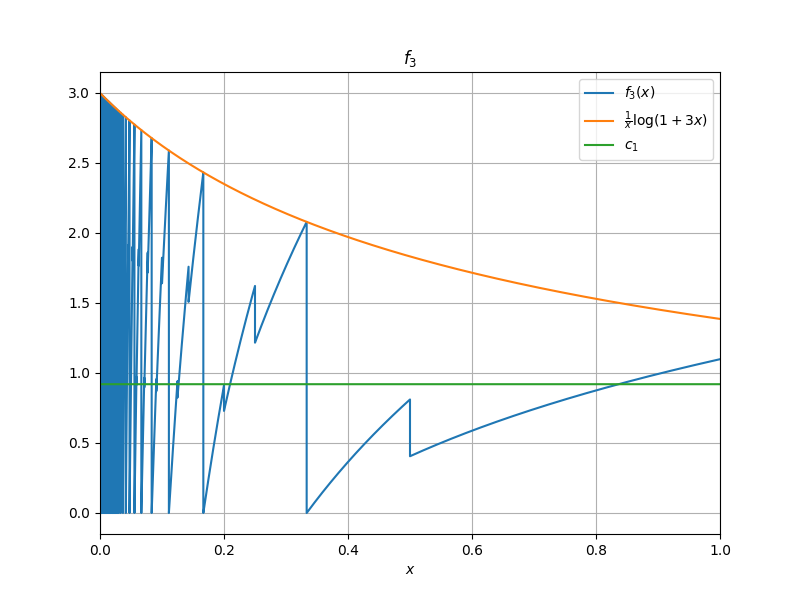
\includegraphics[width=0.5\textwidth]{discrepancy.png}
  \caption{A plot of $f(x)$.  The integral $c_1 = \int_{1/K}^1 f(x)\ dx \approx 0.9200$ is slightly larger than $ec_0 \approx 0.8244$.}
  \label{fig-f}
  \end{figure}

We can directly compute $\pi(K)-\pi(3) = 66$.



\appendix

\section{Powers of 2 and 3}\label{power-sec}

We now obtain good bounds on the quantity $\kappa_L$ introduced in \eqref{kappa-def}.  Clearly $\kappa_L$ is a non-increasing function of $L$ with $\kappa_1 = \log 2$.  The following lemma gives improved control on $\kappa_L$ for large $L$:

\begin{lemma}\label{lemcount-0}  If $n_1,n_2,m_1,m_2$ are natural numbers such that $n_1+n_2, m_1+m_2 \geq 1$ and
$$ 1 \leq \frac{3^{m_1}}{2^{n_1}}, \frac{2^{n_2}}{3^{m_2}}$$
then
$$ \kappa_{\min( 2^{n_1+n_2},3^{m_1+m_2})/6} \leq \log \max\left(\frac{3^{m_1}}{2^{n_1}}, \frac{2^{n_2}}{3^{m_2}}\right).$$
\end{lemma}

\begin{proof}  If $\min( 2^{n_1+n_2},3^{m_1+m_2})/6 \leq t \leq 2^{n_2-1} 3^{m_1-1}$, then we have
\begin{equation}\label{tb} 
  t \leq 2^{n_2-1} 3^{m_1-1} \leq \max\left(\frac{3^{m_1}}{2^{n_1}}, \frac{2^{n_2}}{3^{m_2}}\right) t,
\end{equation}
so we are done in this case.  Now suppose that $t > 2^{n_2-1} 3^{m_1-1}$.
If we write $\lceil t \rceil^{\langle 2,3 \rangle} =2^n 3^m$ be the smallest $3$-smooth number that is at least $t$, then we must have $n \geq n_2$ or $m \geq m_1$ (or both).  Thus at least one of $\frac{2^{n_1}}{3^{m_1}} 2^n 3^m$ and $\frac{3^{m_2}}{3^{n_2}} 2^n 3^m$ is an integer, and is thus at most $t$ by construction.  This gives \eqref{tb}, and the claim follows.
\end{proof}

Some efficient choices of parameters for this lemma are given in \Cref{approx-table}.  For instance, $\kappa_{4.5} \leq 0.28768\dots$ and $\kappa_{40.5} \leq 0.16989\dots$.

\begin{table}[ht]
\centering
\begin{tabular}{|c|c|c|c|c|c|}
\hline
$n_1$ & $m_1$ & $n_2$ & $m_2$ & $\min(2^{n_1+n_2},3^{m_1+m_2})/6$ & $\log \max(3^{m_1}/2^{n_1}, 2^{n_2}/3^{m_2})$ \\
\hline
$1$ & $1$ & $\mathbf{1}$ & $\mathbf{0}$ & $1/2 = 0.5$ & $\log 2 = 0.69314\dots$ \\
\hline
$\mathbf{1}$ & $\mathbf{1}$ & $2$ & $1$ & $2^2/3 = 1.33\dots$ & $\log (3/2) = 0.40546\dots$\\
\hline
$3$ & $2$ & $\mathbf{2}$ & $\mathbf{1}$ & $3^2/2 = 4.5$ & $\log (2^2/3) = 0.28768\dots$ \\
$3$ & $2$ & $\mathbf{5}$ & $\mathbf{3}$ & $3^4/2 = 40.5$ & $\log (2^5/3^3) = 0.16989\dots$ \\
\hline
$\mathbf{3}$ & $\mathbf{2}$ & $8$ & $5$ & $2^{10}/3 = 341.33\dots$ & $\log (3^2/2^3) = 0.11778\dots$\\ 
$\mathbf{11}$ & $\mathbf{7}$ & $8$ & $5$ & $2^{18}/3 = 87381.33\dots$ & $\log (3^7/2^{11}) = 0.06566\dots$ \\
\hline
$19$ & $12$ & $\mathbf{8}$ & $\mathbf{5}$ & $3^{17}/2 \approx 6.4 \times 10^7$ & $\log (2^8/3^5) = 0.05211\dots$ \\
$19$ & $12$ & $\mathbf{27}$ & $\mathbf{17}$ & $3^{29}/2 \approx 3.4 \times 10^{13}$ & $\log (2^{27}/3^{17}) = 0.03856\dots$ \\
$19$ & $12$ & $\mathbf{46}$ & $\mathbf{29}$ & $3^{41}/2 \approx 1.8 \times 10^{19} $ & $\log (2^{46}/3^{29}) = 0.02501\dots$ \\
\hline
\end{tabular}
\caption{Efficient parameter choices for \Cref{lemcount-0}.  The parameters used to attain the minimum or maximum are indicated in \textbf{boldface}. Note how the number of rows in each group matches the terms $1,1,2,2,3,\dots$ in the continued fraction expansion.}\label{approx-table}
\end{table}

\begin{remark}
It should be unsurprising that the continued fraction convergents $1/1$, $2/1$, $3/2$, $8/5$, $19/12$, $\dots$ to 
$$\frac{\log 3}{\log 2} = 1.5849\dots = [1; 1,1,2,2,3,1,\dots]$$
are often excellent choices for $n_1/m_1$ or $n_2/m_2$, although other approximants such as $5/3$ or $11/7$ are also usable.
\end{remark}

Asymptotically, we have logarithmic-type decay:

\begin{lemma}[Baker bound]\label{baker} We have
  $$ \kappa_L \ll \log^{-c} L$$
for all $L \geq 2$ and some absolute constant $c>0$.
\end{lemma}


\begin{proof}  From the classical theory of continued fractions, we can find rational approximants
\begin{equation}\label{abn}
 \frac{p_{2j}}{q_{2j}} \leq \frac{\log 3}{\log 2} \leq \frac{p_{2j+1}}{q_{2j+1}}
\end{equation}
to the irrational number $\log 3/\log 2$, where the convergents $p_j/q_j$ obey the recursions
$$ p_j = b_j p_{j-1} + p_{j-2}; \quad q_j = b_j q_{j-1} + q_{j-2}$$
with $p_{-1} = 1, q={-1}=0, p_0 = b_0, q_0=1$, and 
$$[b_0;b_1,b_2,\dots] = [1;1,1,2,2,3,1\dots]$$ 
is the continued fraction expansion of $\frac{\log 3}{\log 2}$.  Furthermore, $p_{2j+1}q_{2j} - p_{2j} q_{2j+1} = 1$, and hence
\begin{equation}\label{abn-2} 
  \frac{\log 3}{\log 2} - \frac{p_{2j}}{q_{2j}} = \frac{1}{q_{2j} q_{2j+1}}.
\end{equation}
By Baker's theorem, $\frac{\log 3}{\log 2}$ is a Diophantine number, giving a bound of the form
\begin{equation}\label{bj1}
   q_{2j+1} \ll q_{2j}^{O(1)}
\end{equation}
and a similar argument (using $p_{2j+2} q_{2j+1}-p_{2j+1} q_{2j+2} = -1$) gives
\begin{equation}\label{bj2}
 q_{2j+2} \ll q_{2j+1}^{O(1)}.
\end{equation}
We can rewrite \eqref{abn} as
$$ 1 \leq \frac{3^{q_{2j}}}{2^{p_{2j}}}, \frac{2^{p_{2j+1}}}{3^{q_{2j+1}}}$$
and routine Taylor expansion using \eqref{abn-2} gives the upper bounds
$$ \frac{3^{q_{2j}}}{2^{p_{2j}}}, \frac{2^{p_{2j+1}}}{3^{q_{2j+1}}}\leq \exp\left( O\left( \frac{1}{q_{2j}}\right)\right).$$
From \Cref{lemcount-0} we obtain
$$
\kappa_{\min(2^{p_{2j} + p_{2j+1}}, 3^{q_{2j}+q_{2j+1}})/6} \ll \frac{1}{q_{2j}}.$$
The claim then follows from \eqref{bj1}, \eqref{bj2} after optimizing in $j$.

\end{proof}


It seems reasonable to conjecture that $c$ can be taken to be arbitrarily close to $1$, but this is essentially equivalent to the open problem of determining that irrationality measure of $\log 3 / \log 2$ is equal to $2$.


\section{Key inequality}\label{key-app}

We now prove \Cref{key-ineq}. Writing $\nu_p(m) = \sum_{j \geq 1} 1_{p^j|m}$, it suffices to show that
  $$ 0 \leq \sum_{m \leq K; (m,6)=1, p^j|m} \frac{3}{m}
  - \sum_{m \leq K, p^j|m} \log \frac{m}{m-1} \leq \frac{2}{p^j}$$
  for all $j$.  Making the change of variables $m = p^j n$, it suffices to show that
  $$ 0 \leq \sum_{n \leq K'} \frac{3}{n} 1_{(n,6)=1} - p^j \log \frac{p^j n}{p^j n - 1} \leq 2$$
  for any $K' > 0$.   Using the bound
  $$ \log \frac{p^jn}{p^jn - 1} = \int_{p^jn-1}^{p^jn} \frac{dx}{x} \in [\frac{1}{p^j n}, \frac{1}{p^jn-1}]$$
  and $p^j \geq 5$, we have
  $$ \frac{1}{n} \leq p^j \log \frac{p^j n}{p^j n - 1} \leq \frac{1}{n-0.2}$$
  and so it suffices to show that
  \begin{equation}\label{kb}
  0 \leq \sum_{n \leq K'} \frac{3}{n} 1_{(n,6)=1} - \frac{1}{n-0.2} 
  \leq
  \sum_{n \leq K'} \frac{3}{n} 1_{(n,6)=1} - \frac{1}{n} \geq 2.
  \end{equation}
  Since 
  $$ \sum_{n=1}^\infty \frac{1}{n-0.2}-\frac{1}{n} = \psi(0.8)-\psi(1) = 0.353473,$$
  where $\psi$ here denotes the digamma function rather than the von Mangoldt summatory function, it will suffice to show that
  \begin{equation}\label{kb-2} 0.4 \leq
  \sum_{n \leq K'} \frac{3}{n} 1_{(n,6)=1} - \frac{1}{n} \geq 2.\end{equation}
  This can be numerically verified for $K' \leq 100$, with substantial room to spare for $K'$ large; see \Cref{fig:kb}. On a block $6a-1 \leq n \leq 6a+4$, the sum is positive:
  \begin{align*}
  \sum_{6a-1 \leq n \leq 6a+4} \frac{3}{n} 1_{(n,6)=1} - \frac{1}{n } &= \left(\frac{1}{6a-1} - \frac{1}{6a}\right) + \left(\frac{1}{6a-1} - \frac{1}{6a+2}\right)\\
  &\quad + \left(\frac{1}{6a+1} - \frac{1}{6a+3}\right) + \left(\frac{1}{6a+1} - \frac{1}{6a+4}\right) \\
  &\quad > 0.
  \end{align*}
  Similarly, on a block $6a-4 \leq n \leq 6a+1$, the sum is negative:
  \begin{align*}
    \sum_{6a-4 \leq n \leq 6a+1} \frac{3}{n} 1_{(n,6)=1} - \frac{1}{n } &= \left(\frac{1}{6a+1} - \frac{1}{6a}\right)
    + \left(\frac{1}{6a+1} - \frac{1}{6a-2}\right)\\
    &\quad  + \left(\frac{1}{6a-1} - \frac{1}{6a-3}\right)
    + \left(\frac{1}{6a-1} - \frac{1}{6a-4}\right)\\
    &\quad  < 0.
  \end{align*}
  Thus the sum in \eqref{kb-2} is increasing for $K' = 4\ (6)$ and decreasing for $K' = 1\ (6)$, and the inequality for $K'>100$ is then easily verified from the $K' \leq 100$ data and the triangle inequality
  
    From this and the triangle inequality one can easily establish \eqref{kb} in the remaining ranges $K' \geq 98$.
  
  \begin{figure}
  \centering
  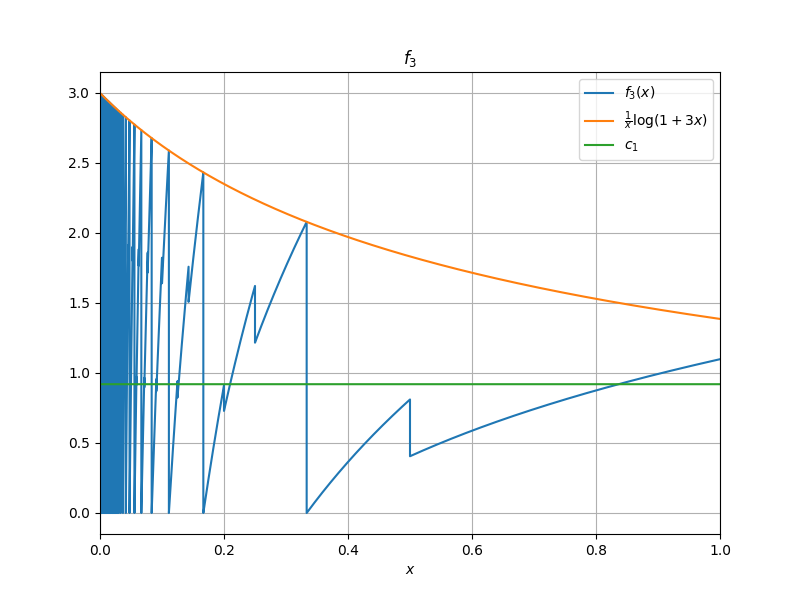
\includegraphics[width=0.5\textwidth]{discrepancy.png}
  \caption{A plot of \eqref{kb}.}
  \label{fig:kb}
  \end{figure}

\section{Estimating sums over primes}\label{primes-sec}

In this section we collect some estimates on sums over primes from the literature that we will use in this paper.

We recall the effective prime number theorem from \cite[Corollary 5.2]{dusart}, which asserts that
\begin{equation}\label{pi-lower}
  \pi(x) \geq \frac{x}{\log x} + \frac{x}{\log^2 x}
\end{equation}
for $x \geq 599$ and
\begin{equation}\label{pi-upper}
  \pi(x) \leq \frac{x}{\log x} + \frac{1.2762 x}{\log^2 x}
\end{equation}
for $x >1$.  


\begin{lemma}[Integration by parts]\label{integ-lemma}  Let $(y,x]$ be a half-open interval in $(0,+\infty)$.  Suppose that one has a function $a \colon \N \to \R$ and a continuous function $f: (y,x] \to \R$ such that 
  $$ \sum_{y < n \leq z} a_n = \int_z^y f(t)\ dt + C + O_{\leq}(A)$$
  for all $y \leq z \leq x$, and some $C \in \R$, $A>0$.  Then, for any function $b: (y,x] \to \R$ of bounded total variation, one has
\begin{equation}\label{tve}
   \sum_{y < n \leq x} b(n) a_n = \int_x^y b(t) f(t)\ dt + O_{\leq}(A\|b\|_{\mathrm{TV}^*(y,x]}),
\end{equation}
where the augmented total variation $\|b\|_{\mathrm{TV}^*(y,x]}$ is defined as
$$
\|b\|_{\mathrm{TV}^*(y,x]}
\coloneqq |b(y^+)| + |b(x)| + \|b\|_{\mathrm{TV}(y,x]},$$
$b(y^+) \coloneqq \lim_{t \to y^+} b(t)$ denotes the right limit of $b$ at $y$, and the total variation $\|b\|_{\mathrm{TV}(y,x]}$ is defined as the supremum of the quantities $\sum_{j=0}^{J-1} |b(x_{j+1})-b(x_j)|$ for $y < x_0 \leq \dots \leq x_J \leq x$.
\end{lemma}

\begin{proof}  If, for every natural number $y < n \leq x$, one modifies $b$ to be equal to the constant $b(n)$ in a small neighborhood of $n$, then one does not affect the left-hand side of \eqref{tve} or increase the total variation of $b$, while only modifying the integral in \eqref{tve} by an arbitrarily small amount.  Hence, by the usual limiting argument, we may assume without loss of generality that $b$ is locally constant at each such $n$.  If we define the function $g \colon (y,x] \to \R$ by
$$ g(z) \coloneqq  \sum_{y < n \leq z} a_n - \int_z^y f(u)\ du - C$$
then $g$ has jump discontinuities at the natural numbers, but is otherwise continuously differentiable, and is also bounded uniformly in magnitude by $A$.  We can then compute the Riemann--Stieltjes integral
$$ \int_{(y,x]} b\ dg = \sum_{y < n \leq x} b(n) a_n - \int_y^x f(t) b(t)\ dt.$$
Since the discontinuities of $g$ and $b$ do not coincide, we may integrate by parts to obtain
$$ \int_{(y,x]} b\ dg = b(x) g(x) - b(y^+) g(y^+) - \int_{(y,x]} g db.$$
The left-hand side is $O_{\leq}(A \|b\|_{\mathrm{TV}^*(y,x]})$, and the claim follows.
\end{proof}

By combining this lemma with effective prime number estimates, we obtain

\begin{lemma}[Effective prime number theorem]\label{buthe}  Under the above hypotheses 
with $1423 \leq y \leq x$, one has
$$  \sum_{y < p \leq x} b(p) \log p = \int_y^x b(t) (1 - \frac{2}{\sqrt{t}}) \ dt
+ O_\leq\left(\|b\|_{\mathrm{TV}^*((y,x])} E(x) \right)$$
where
$$
E(x) \coloneqq 0.95 \sqrt{x} + \frac{\sqrt{x}}{8\pi} \log x(\log x - 3) 1_{x \geq 10^{19}} + \min( \eps_0, \eps_1(x), \eps_2(x)) x 1_{x \geq e^{45}}$$
and
\begin{align*}
  \eps_0 &\coloneqq 1.11742 \times 10^{-8}\\
  \eps_1(x) &\coloneqq 9.39 (\log^{1.515} x) \exp(-0.8274\sqrt{\log x})\\
  \eps_2(x) &\coloneqq 0.026 (\log^{1.801} x) \exp(-0.1853 (\log^{3/5} x) (\log\log x)^{-1/5})
\end{align*}
  for some absolute constant $c>0$.
\end{lemma}

\begin{proof} Observe that $E$ is monotone non-decreasing. Thus by \Cref{integ-lemma}, it will suffice to show that
$$ \sum_{p \leq x} \log p = x - \sqrt{x} + O_{\leq}(E(x))
  = \int_0^x \left(1-\frac{2}{\sqrt{t}}\right)\ dt + O_{\leq}(E(x))$$
for all $x \geq 1423$.

For $1423 \leq x \leq 10^{19}$, this follows from \cite[Theorem 2]{buthe-2}.  In the range
For $10^{19} \leq x \leq 10^{21} \approx e^{48.35}$, we use the bound
  $$ \psi(x) = x + O_{\leq}\left(\frac{\sqrt{x}}{8\pi} \log x(\log x - 3)\right)
$$
which was established for $5000 \leq x \leq 10^{21}$ in \cite[(7.3)]{buthe}, where $\psi(x) \coloneqq \sum_{n \leq x} \Lambda(n)$ is the usual von Mangoldt summatory function.  To use this, we apply \cite[(6.10), (6.11)]{buthe} to conclude that
$$
\sum_{p \leq x} \log p = \psi(x) - \psi(\sqrt{x}) + O_{\leq}(1.03883 (x^{1/3} + x^{1/5} + 2 (\log x) x^{1/13})).$$
From \cite[Theorems 10,12]{rs} we have
$$ \psi(\sqrt{x}) = \sqrt{x} + O_{\leq}(0.18 \sqrt{x}).$$
Since
$$ 0.18 \sqrt{x} + 1.03883 (x^{1/3} + x^{1/5} + 2 (\log x) x^{1/13}) \leq 0.95 \sqrt{x}$$
for $x \geq 10^{19}$, the claim follows.

Finally, in the range $x \geq 10^{21}$, we see from \cite[Theorem 1, Table 1]{buthe} that one has the bound
$$ \psi(x) = x + O_{\leq}(\eps_0)$$
for $x \geq e^{45} \approx 10^{19.54}$, while from \cite[Theorems 1.1, 1.4]{johnston-yang} one has
$$ \psi(x) = x + O_{\leq}(\eps_1(x))$$
and
$$ \psi(x) = x + O_{\leq}(\eps_2(x))$$
for all $x \geq 2$.  The claim then follows by repeating the previous arguments.
\end{proof}
    
\begin{remark} Assuming the Riemann hypothesis, the final term in the definition of $E(x)$ may be deleted, since \cite[(7.3)]{buthe} then holds for all $x \geq 5000$.  
\end{remark}

Applying the above lemma to $b(t) = 1/\log t$, we conclude in particular that
\begin{equation}\label{pi-est} \pi(x) - \pi(y) = \int_y^x(1 - \frac{2}{\sqrt{t}}) \ \frac{dt}{\log t}
+ O_\leq(\frac{2 E(x)}{\log y})
\end{equation}
for $1423 \leq y \leq x$. In particular, we have the slightly crude upper bound
\begin{equation}\label{pixy-upper} \pi(x) - \pi(y) \leq \frac{x-y}{\log y} + \frac{2 E(x)}{\log y}
\end{equation}
in this range, as well as the lower bound
\begin{equation}\label{pixy-lower} \pi(x) - \pi(y) \geq \left(1-\frac{2}{\sqrt{y}}\right)\frac{x-y}{\log y} - \frac{2 E(x)}{\log y}
\end{equation}

The quantity $E(x)$ is somewhat complicated.  In our paper we will only need simpler upper bounds on this quantity.  Firstly, from the $\eps_1$ term we obtain the classical error term
\begin{equation}\label{ecx}
E(x) \ll x \exp(-c \sqrt{\log x})
\end{equation}
for some absolute constant $c>0$.  Secondly, because
$$ \frac{\log x (\log x-3)}{8\pi\sqrt{x}}  \leq 2.244 \times 10^{-8}$$
for $x \geq 10^{19}$, we also have the upper bound
\begin{equation}\label{ecx-2}
E(x) \leq \tilde E(x)
\end{equation}
where
\begin{equation}\label{tilde-e}
  \tilde E(x) \coloneqq 0.95 \sqrt{x} + 2.25 \times 10^{-8} x.
\end{equation}
One small advantage of working with $\tilde E$ instead of $E$ is that in addition to being monotone increasing, $\tilde E(x)/x$ is monotone decreasing.



  


\section{Computation of \texorpdfstring{$c_0$}{c\_0}}\label{c0-app}

In this appendix we give some details regarding the rigorous numerical estimation of the constant $c_0$ defined in \eqref{c0-def}.  As one might imagine from an inspection of \Cref{fig-mean}, direct application of numerical quadrature converges quite slowly due to the oscillatory singularity.  To resolve the singularity, we can perform a change of variables $x=1/y$ to express $c_0$ as an improper integral:
\begin{equation}\label{c0-alt}
   c_0 = \frac{1}{e} \int_1^\infty \lfloor y \rfloor \log \frac{\lceil y/e \rceil}{y/e}\ \frac{dy}{y^2}.
\end{equation}
The integrand is piecewise smooth and the integral can be computed explicitly on any interval $[a,b]$ of the form
$$ [a,b] \subset [n, n+1] \cap [(m-1)e, me]$$
for some non-negative integers $n,m$ as
$$ \int_a^b \lfloor y \rfloor \log \frac{\lceil y/e \rceil}{y/e}\ \frac{dy}{y^2} = n (\frac{\log(b/m)}{b} - \frac{\log(a/m)}{a}).$$
This formula permits one to evaluate $\int_1^b \lfloor y \rfloor \log \frac{\lceil y/e \rceil}{y/e}\ \frac{dy}{y^2}$ exactly for any finite $b$.  To control the tail, we see from the crude bounds $0 \leq \lfloor y \rfloor \leq y$ and
$$ 0 \leq \log \frac{\lceil y/e \rceil}{y/e} \leq \log 
\left(1 + \frac{e}{y}\right) \leq \frac{e}{y}
$$
that
\begin{equation}\label{tail}
   0 \leq \int_b^\infty \lfloor y \rfloor \log \frac{\lceil y/e \rceil}{y/e}\ \frac{dy}{y^2} \leq \frac{e}{b}
\end{equation}
which allows for rigorous upper and lower bounds on the improper integral.  For instance, this procedure gives
$$ 0.304419004 \leq c_0 \leq 0.304419017.$$
Heuristically, the tail integral \eqref{tail} should be approximately $e/2b$ due to the equidistribution properties of the fractional part of $y/e$.  Using this heuristic approximation, one obtains the prediction
$$ c_0 \approx 0.30441901087.$$
It should be possible to obtain this level of precision more rigorously (using interval arithmetic to preclude any possibility of roundoff error), but we have not attempted to do so.

\begin{thebibliography}{10}

  
\bibitem{algr77}
K. Alladi, C. Grinstead, \emph{On the decomposition of $n!$ into prime powers}, J. Number Theory \textbf{9} (1977) 452--458.

\bibitem{bincover}
S. F. Assmann, D. S. Johnson, D. J. Kleitman, J. Y.-T. Leung, \emph{On a dual version of the one-dimensional bin packing problem}, J. Algorithms \textbf{5} (1984) 502--525.

\bibitem{buthe}
J. B\"uthe, \emph{Estimating $\pi(x)$ and related functions under partial RH assumptions}, Math. Comp., 85(301), 2483--2498, Jan. 2016.

\bibitem{buthe-2}
J. B\"uthe, \emph{An analytic method for bounding $\psi(x)$
}. Math. Comp., \textbf{87} (312), 1991--2009.


%\bibitem{dusart}
%P. Dusart, \emph{In\'egalit\'es explicites pour $\psi(x)$, $\theta(x)$, $\pi(x)$ et les nombres premier}, C. R. Math. Rep. Acad. Sci. Canada Vol. \textbf{21} (2) 1999, pp. 53--59.


\bibitem{dusart}
P. Dusart, \emph{Explicit estimates of some functions over primes}, Ramanujan J. \textbf{45} (2018) 227--251.

\bibitem{erdos-71}
P. Erd\H{o}s, \emph{Some problems in number theory}, in Computers in Number Theory, Academic Press, London New York, 1971, pp. 405--414.

\bibitem{erdos-96}
P. Erd\H{o}s, \emph{Some problems I presented or planned to present in my short talk}, Analytic number theory, Vol. 1 (Allerton Park, IL, 1995) (1996), 333--335.

\bibitem{erdos-graham}
P. Erd\H{o}s, R. Graham, \emph{Old and new problems and results in combinatorial number theory}, Monographies de L'Enseignement Mathematique 1980.

\bibitem{guy}
R. K. Guy, \emph{Unsolved Problems in Number Theory}, 3rd Edition, Springer, 2004.

\bibitem{guy-selfridge}
R. K. Guy, J. L. Selfridge, \emph{Factoring factorial $n$}, Amer. Math. Monthly \textbf{105} (1998) 766--767.

\bibitem{johnston-yang}
D. Johnston, A. Yang, \emph{Some explicit estimates for the error term in the prime number theorem}, J. Math. Anal. Appl., \textbf{527} (2) (2023), Paper No. 127460.

\bibitem{robbins}
H. Robbins, \emph{A Remark on Stirling's Formula}, Amer. Math. Monthly \textbf{62} (1955) 26--29.

%\bibitem{faber-kadiri}
%L. Faber, H. Kadiri, \emph{Corrigendum to: New bounds for $\psi(x)$}, Math. Comp. \textbf{87} (2018) 1451--1455.

\bibitem{rs}
J. Rosser, L. Schoenfeld, \emph{Approximate formulas for some functions of prime numbers}, Illinois J. Math. 6 (1962), 64--94.

\bibitem{tao}
T. Tao, \emph{Decomposing factorials into bounded factors}, preprint, 2025. \url{https://arxiv.org/abs/2503.20170v2}

\bibitem{github}
T. Tao, \emph{Verifying the Guy--Selfridge conjecture}, Github repository, 2025.  \url{https://github.com/teorth/erdos-guy-selfridge}.

\end{thebibliography}


\end{document}
